%!TEX root = ../thesis.tex

\chapter{Results}
\textit{Parts of this section incorporate text from published work [The central complex of the larval fruit fly brain] (Lungu et al., 2025)}


\section{Strategy for identifying CX neuropils in the larval brain}

    I used an iterative strategy in finding putative larval central complex neurons. For this, I pattern matched individual cells based on adult CX neurons lineages, morphology, relative location and connectivity. %describe the steps of the process at a bit more length 
    %We adopted a search strategy guided by circuit features of the adult brain CX neuropils.
    Since the adult brain presents fused hemispheres at the midline whereas the larva has not, we placed more emphasis of searching for circuit motifs rather than anatomical similarity, since the larval brain has a brain commisure, while preserving the relative spatial location of a CX neuropil as a constraint.

    These included:
    \begin{enumerate}
    \item Integration of sensory inputs: we searched for synaptic pathways corresponding to the adult's for integrating visual inputs into the PB and EB \citep{hulse2021connectome}, and gustatory inputs into the FB.
    \item Association between centers for memory and spatial navigation: we looked for the characteristic link between the MB, the center for associative memory, and CX neuropils, which includes synapses from MBONs (MB output neurons) to the FB, EB and NO in the adult fly.
    \item Recurrent intra-CX connectivity, such as with columnar neurons relating the PB with the FB and EB, or with the NO.
    \end{enumerate}
    
    \subsection{Identifying larval neuronal lineages that contribute to the larval CX}
    The \textit{Drosophila melanogaster} central brain consists of stereotyped neural lineages, developmental-structural units of macrocircuitry formed by the sibling neurons of single progenitor cells, the neuroblasts \citep{Spindler2010Lineages}, a subset of which structures the CX \citep{Pereanu2011LineagesCX}.
    Starting with the currently identified set of quiescent, embryonic-born neurons present in the larval brain that develop into to the adult CX during metamorphosis~\citep{andrade2019developmentally}
    we identified larval brain neurons satisfying imposed connectivity rules as per known circuit patterns across the adult CX neuropils \citep{wolff2015neuroarchitecture, wolff2018neuroarchitecture, franconville2018building, hulse2021connectome}.

    We broadened the search beyond these lineages based on the expectation that some larval neurons may have been recruited to CX structures but would later take another identity in the adult, as is known for larval MB neurons \citep{truman2023metamorphosis}, on the basis of matching synaptic connectivity patterns as observed in the adult; for example, for EB Ring neurons we looked for neurons with recurrent axo-axonic synapses with each other and with Wedge neurons, where their axon is located at the most anterior end of the brain neuropil, at an intermediate dorso-ventral position just anterior to the MB medial lobe.
    %MY PART 
    %Lineages
    We expected to find neurons originating from DM1, DM2, DM3, DM4, DM5 and DM6 hemilineages as these are core lineages contributing to all neuropils(Table \ref{adultlineages}), with the second priority being neuropil specific lineages(e.g. EBa1(DALv2) for the EB see \ref{adultlineages}). 12 of the 15 lineages found to contribute CX neurons in the adult also exist in the larva. Of these, we found that 9 of them contribute neurons to the larval central complex (Table \ref{lineagemap}). We therefore used these 9 lineages as a starting point to find our putative CX neuropils in the larva.

        \begin{table}
        \centering
        \begin{tabular}{|c|c|}
        \hline
        Adult lineage & Larval lineage \\
        \hline
        DM1 & DPMm1 \\
        DM2 & DPMpm1 \\
        DM3 & DPMpm2 \\
        DM4 & CM4 \\
        DM5/DM6 & CM1/3 \\
        DL1 & CP23 \\
        EBa1 & DALv2 \\
        LALv1 & BAMv1 \\
        CREa1 & BAmd1 \\
        CREa2 & DALCm12 \\
        SMPad2 & DAMd2/3 \\
        SIPp1 & DPMpl12 \\
        \bottomrule
        \end{tabular}
        \caption[Lineges of the Adult CX that also contribute neurons to the Larval CX]{\textbf{Lineges of the Adult CX that also contribute neurons to the Larval CX} Adult CX lineages are listed in the first column, and their corresponding larval lineages in the second.}
        \label{lineagemap}
        \end{table}

    In addition to the lineages that contribute to the adult CX, there were several neurons from other lineages, which satisfied other criteria (such as connectivity patterns or relative location) and were therefore classified as central complex neurons. These lineages are presented in Table \ref{larvallineages} which containts all the lineages we found to contribute neurons to the larval CX. None of these lineages are exclusive contributors to the larval CX - i.e all of these lineages contribute neurons to other parts of the brain - however, there are a few(about 10) that contribute more than a fifth (20\%) of their neurons to CX neuropils (Figure (\ref{cx_percentage})).


    \begin{table}
    \centering
    \resizebox{\textwidth}{!}{%
    \begin{tabular}{|c|c|c|c|c|c|c|c|c|c|}
    \toprule
    Larval lineages & PB.b & PB.d & FB.b & FB.d & EB.b & EB.d & NO.b & NO.d & Total \\
    \midrule
    BAla12 &  &  &  & 2 & 2 &  &  &  & 4 \\
    BAla34 &  &  & 4 &  &  &  &  & 9 & 13 \\
    BAlp\_ant &  & 2 &  &  & 2 &  &  & 1 & 5 \\
    bamd1 &  &  &  &  &  & 1 &  & 2 & 3 \\
    bamd2\_d &  &  & 1 &  &  &  &  &  & 1 \\
    bamd2\_v &  &  & 3 &  &  &  &  & 4 & 7 \\
    bamv12\_dor & 1 &  &  & 1 &  &  & 2 & 5 & 9 \\
    BAmv12\_dor & 1 &  &  & 1 &  &  & 2 & 5 & 9 \\
    Bamv12\_ven & 1 &  &  & 1 & 2 & 2 &  & 1 & 7 \\
    BLAd-OL & 2 &  &  &  &  &  &  &  & 2 \\
    BLAl &  &  &  & 2 &  &  &  &  & 2 \\
    BLAV12\_ant &  &  &  & 2 &  &  &  &  & 2 \\
    BLP12 &  &  &  &  &  & 2 &  &  & 2 \\
    BLVp2 &  & 2 &  &  &  &  &  &  & 2 \\
    CM13\_lat &  & 2 &  &  & 4 & 2 &  &  & 8 \\
    CM13\_med &  &  &  &  & 2 & 2 &  &  & 4 \\
    CM4-vm &  &  &  & 2 &  &  &  & 4 & 6 \\
    CPa &  &  & 1 &  &  &  &  &  & 1 \\
    CPb &  &  &  &  & 8 & 4 &  &  & 12 \\
    CPe &  &  &  & 2 &  &  &  & 4 & 6 \\
    Dalcl12 &  &  &  &  & 16 & 22 &  &  & 38 \\
    Dalcm12-m &  &  &  &  &  & 4 &  & 2 & 6 \\
    DALcm12-v &  & 2 &  & 2 &  &  & 4 & 1 & 9 \\
    dall1 &  & 2 & 4 &  &  &  &  &  & 6 \\
    Dalv1 & 8 &  &  & 6 &  &  &  &  & 14 \\
    Dalv23 &  &  &  &  & 14 &  &  & 4 & 18 \\
    dplal1-3 &  &  & 2 &  & 3 &  &  &  & 5 \\
    dplc\_post\_med &  & 4 &  & 2 &  &  & 4 &  & 10 \\
    DPLc5 &  & 6 & 1 & 2 &  &  & 3 &  & 12 \\
    DPMl\_ant & 3 & 2 &  &  &  &  &  & 3 & 8 \\
    DPMl12 &  & 3 &  & 2 &  &  & 2 &  & 7 \\
    DPMl34\_post &  &  &  & 1 &  &  & 1 &  & 2 \\
    DPMm1 & 4 &  & 14 & 2 &  &  & 4 &  & 24 \\
    DPMm2 &  & 3 &  & 2 &  & 2 &  &  & 7 \\
    DPMpl12 &  & 5 & 2 & 2 &  &  &  &  & 9 \\
    dpmpl3 &  &  &  &  &  &  &  & 1 & 1 \\
    DPMpm1 &  &  & 4 & 2 &  & 4 &  &  & 10 \\
    DPMpm2 &  &  &  &  &  & 2 & 2 &  & 4 \\
    \bottomrule
    Total & 20 & 33 & 36 & 36 & 53 & 47 & 24 & 46 & 295 \\
    \bottomrule
    \end{tabular}
    }
    \caption[Larval Central Complex Lineages]{\textbf{Larval Central Complex Lineages.} A full list of Larval CX lineages is shown in the first column. If a lineage also contributes to the adult CX, the corresponding adult nomenclature \citep{eckstein2024neurotransmitter} is shown in the second column. Columns 3--6 indicate the number of neurons from each lineage that contribute axons (“.b” for boutons) or dendrites (“.d”) to individual neuropils: PB, FB, EB and NO.}
    \label{larvallineages}
    \end{table}

    % green gradient 
    \definecolor{forest1}{HTML}{EEF4EA} % very light
    \definecolor{forest2}{HTML}{D6E3CB} 
    \definecolor{forest3}{HTML}{B1D19B}
    \definecolor{forest4}{HTML}{84B96F}
    \definecolor{forest5}{HTML}{4C8437} % deep green

    \begin{table}[h!]
    \centering
    \begin{tabular}{|l|c|c|c|c|}
    \hline
    \textbf{Lineage} & \textbf{Left Hemisphere} & \textbf{Right Hemisphere} & \textbf{CX neurons} & \textbf{CX \% of Lineage} \\
    \hline
    Dalcl12 & 25 & 27 & 38 & \cellcolor{forest5}73.08\% \\
    Dalv1 & 11 & 11 & 14 & \cellcolor{forest4}63.64\% \\
    dplc\_post\_med & 6 & 10 & 10 & \cellcolor{forest4}62.50\% \\
    DPMl12 & 13 & 2 & 7 & \cellcolor{forest3}46.67\% \\
    Dalv23 & 18 & 21 & 18 & \cellcolor{forest3}46.15\% \\
    DPLc5 & 13 & 14 & 12 & \cellcolor{forest3}44.44\% \\
    dplal1-3 & 2 & 12 & 5 & \cellcolor{forest2}35.71\% \\
    CPb & 14 & 20 & 12 & \cellcolor{forest2}35.29\% \\
    DPMm1 & 38 & 47 & 24 & \cellcolor{forest1}28.24\% \\
    dall1 & 9 & 18 & 6 & \cellcolor{forest1}22.22\% \\
    \hline
    \end{tabular}
    \caption[Contribution of lineage to CX]{\textbf{Lineage contribution to CX}  This table illustrates lineages that contribute more that 20\% of their neurons ot the CX. the second and third column show their distribution across the brain hemispheres, whilst tha last column shows the percentage of neurons that contribute(axons, dendrites or both) to CX neuropils}
    \label{cx_percentage}
        \end{table}

    \subsection{Connectivity of CX neurons}
    %CONNECTIVITY
    To be able to identify which neurons could contribute to the CX, we investigated their connectivity patterns. Specifically,we summarised where a neuron receives synaptic input (location of its dendrites) and sends output processes (location of its axons).
    %Sensory
    The central complex is known primarily for visual input processing, therefore in the larva we were looked at neurons downstream of photoreceptors. We investigated cells immediately connected to visual projection neurons (vPNs) which are directly connected to photoreceptors. Several of these neurons have been catalogued as Protocerebral Bridge (see section \ref{PB}) or Noduli(see section \ref{NO}) neurons. 
    In additon to visual input, we find that olfactory input is integrated by all the larval CX neuropils indirectly via the Lateral Horn(LH) and the Mushroom Body through convergence neurons(CNs; which integrate learnt valences from the MB and innate valences from the LH \citep{eschbach2021circuits}) or MB output neurons and MB input neurons. This is in line with previous findings about the CX being integrative across multiple sensory modalities \citep{hulse2021connectome}. Since Gepner et al., 2015 demonstrated that Larvae  have to integrate visual and olfactory gradients, with convergence of these sensory systems before decision to act on themwe expected there would be a structure recieving input from these modalities and used information such as lineage membership to figure out if these could be central complex neurons. 

    %Input from other neuropils/lal
    Columnar and horizontal neurons have stereotyped connectivity patterns within the CX, being connected between themselves or with other accessory structures (e.g.LAL). To be able to define these, we categorised them similarly to how they have been categorised in the literature. For naming, we adapted Wolff et al., 2015 nomenclature, and named them on the baisis of the location of input synapses (.d for dendrites) and the location of their output synapses (.b for axonal bouttons). Once the synapses for each neuron was mapped, we categorised them on the basis of their location within the CX neuropils and relative to accesory structures as per Figure \ref{CXclasses}.  As such we devided them into Intrinsic Neurons(those whose inputs and outputs are located within CX neuropils), Local Neurons (cells whose inputs and outputs located within the same neuropil), Input Neurons (those that send only dendrites processes within the CX and output outside of it) and Output Neurons: Cells that send denritic inputs outside of the CX but output onto the CX neuropils. Since the CX of the larva is numerically reduced, we grouped Intrinsic and Local neurons, and named these \textbf{Core CX neurons} for a more concise, cohesive analysis of the CX network. There are 15 pairs of CX core neurons, all of which are presented in Table \ref{CXCoreNeurons}. For a comprehensive understanding of the connectivity patterns of these neurons, they have been written in a nomenclature adapted from Wolff et al., 2015 \citep{wolff2015neuroarchitecture}. We classified neurons using the suffixes ".b" (axon boutons) and ".d" (dendrites) for CX neuropils.
    Hence, a neuron annotated as NO.b projects its axon into the NO, and likewise, a neuron annotated as FB.d places its dendrites in the FB.
    As such, neurons that are both .b and .d for CX neuropils are the CX Core neurons. 



            \begin{figure}
                \centering
                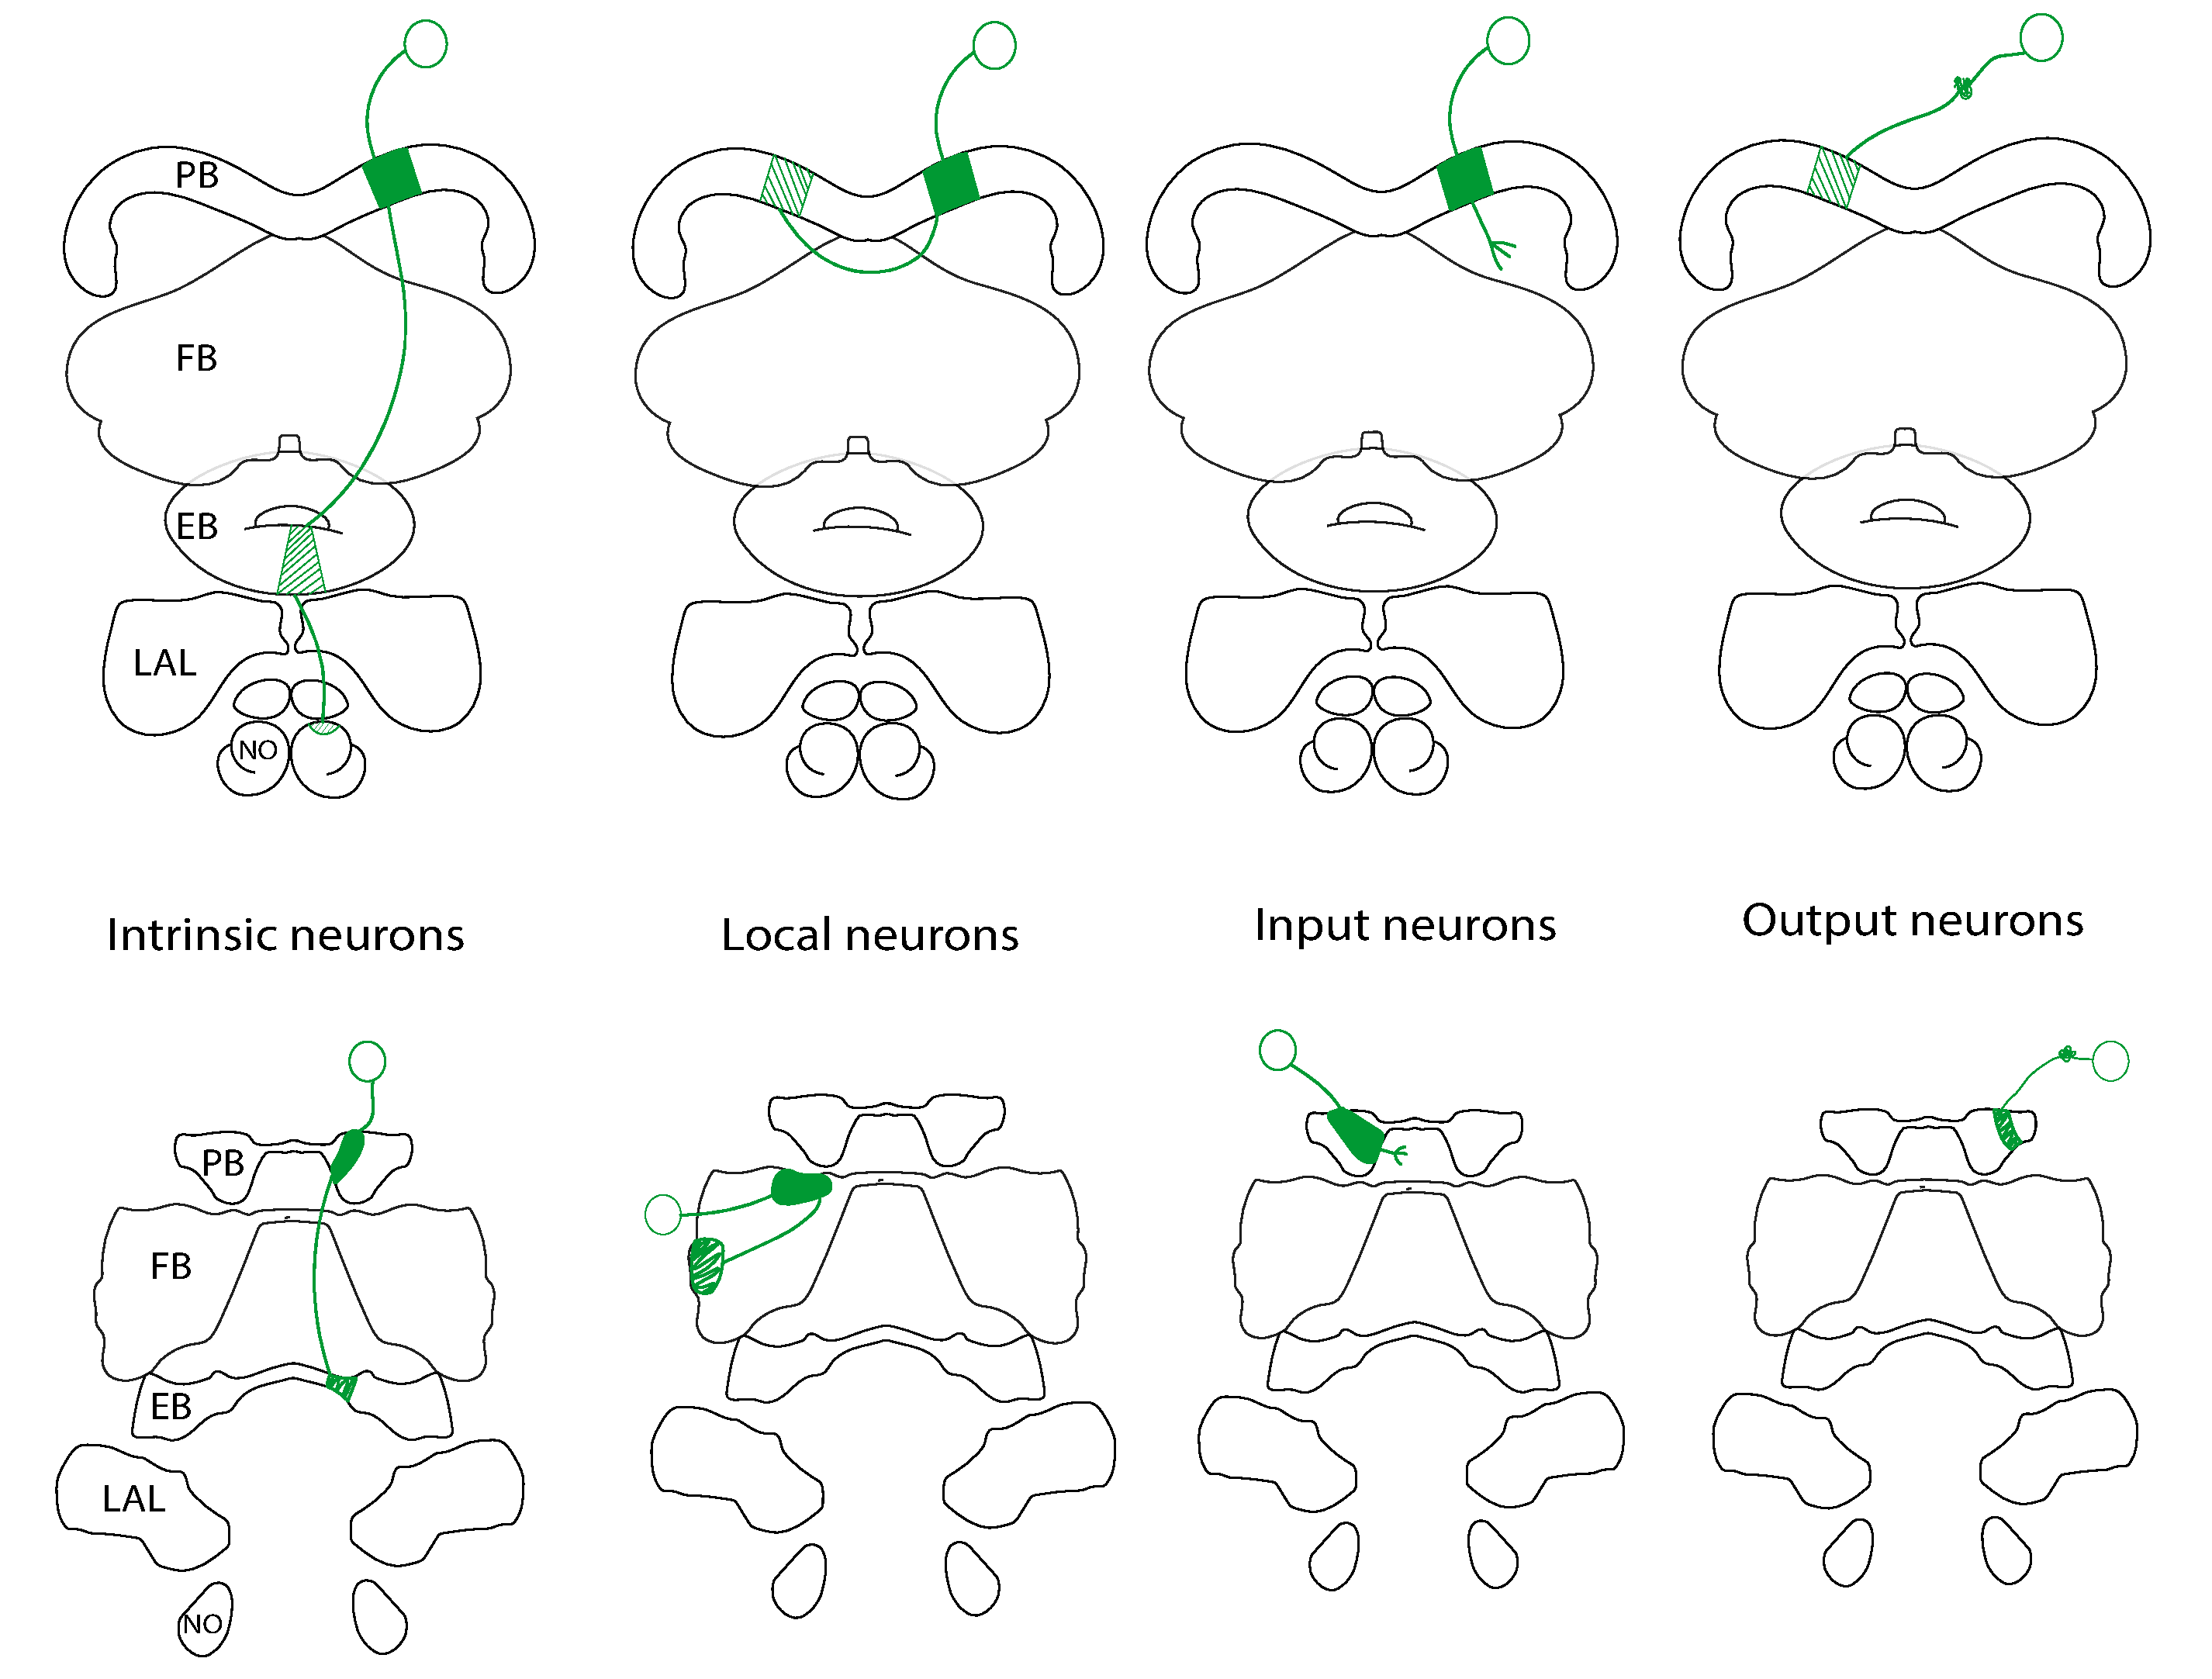
\includegraphics[width=12cm]{Figs/CX/CX_Nomenclature_Neurons.pdf}
                \caption[Central Complex Neuron Classes]{\textbf{Classes of CX neurons} This schematic illustrates neuron classes of the adult CX (upper panel) and the larval CX (lower panel). The PB, FB, EB, NO and LAL are shown in each case to illustrate where a neuron arborizes. Neurons are drawn as a sketch, where the soma is represented by a green circle, the arbors are split into dendritic inputs - filled green boxed - and spiny axonal outputs - hashed scribbled green boxes. Cells are classified as either \textbf{Intrinsic Neurons}:neurons whose inputs and outputs are located within CX neuropils; \textbf{Local Neurons}: cells whose inputs and outputs located within one neuropil; \textbf{Input Neurons}: Neurons that have  dendrites (receive synaptic input) located within the CX but output outside of it; and \textbf{Output Neurons}: Cells that receive inputs outside of the CX but output onto CX neuropils}
                \label{CXclasses}
            \end{figure}

            \begin{table}[h!]
            \centering
            \begin{tabular}{|l|l|}
            \hline
            \textbf{CX Core Neurons} & \textbf{Other Names (CX or MB)} \\
            \hline
            FB.d, NO.b & FB-NO 1, FB.d.1 \\
            FB.d, PB.d, NO.b & FB.d.1, CN-34, MB2ON-119 \\
            FB.d, PB.d, NO.b & FB.d.1, MB2ON-204 \\
            FB.d, NO.b & FB.d.1, MB2ON-201 \\
            EB.d, EB.b, LAL.b & MB2IN-124, MB2ON-79 \\
            EB.d, LAL.d, EB.b & RN4, FBN-19, MB2IN-37, MB2ON-112 \\
            EB.d, LAL.d, EB.b & RN4, FBN-21, MB2IN-42, MB2ON-128 \\
            EB.d, EB.b & RN3, MB2IN-122, MB2ON-71 \\
            EB.d, EB.b & RN1/2a, FBN-20, MB2IN-38, MB2ON-115 \\
            EB.d, EB.b & RN1/2b, FB2IN-10, MB2IN-68, MB2ON-266 \\
            FB.d, FB.b & eDAN-2 \\
            FB.d, FB.b & MB2ON-125 \\
            FB.d, LAL.b & FB.d.2 \\
            PB.d, FB.d & FB.d.2 \\
            PB.d, NO.b & MB2ON-241 \\
            \hline
            \end{tabular}
            \caption[CX Core Neurons]{\textbf{CX Core Neurons} The table illustrates, in the first column, the CX Core neurons in nomenclature adapted from Wolff et al., 2015\citep{wolff2018neuroarchitecture}, depicting the location of the dendrites (.d) axonal butons (.b) in the Central Complex Neuropils. Each neuron is listed alongside their CX neuropil-specific nomenclature, and/or their MB nomenclature}
            \label{CXCoreNeurons}
            \end{table}



    \begin{figure}
        \centering
        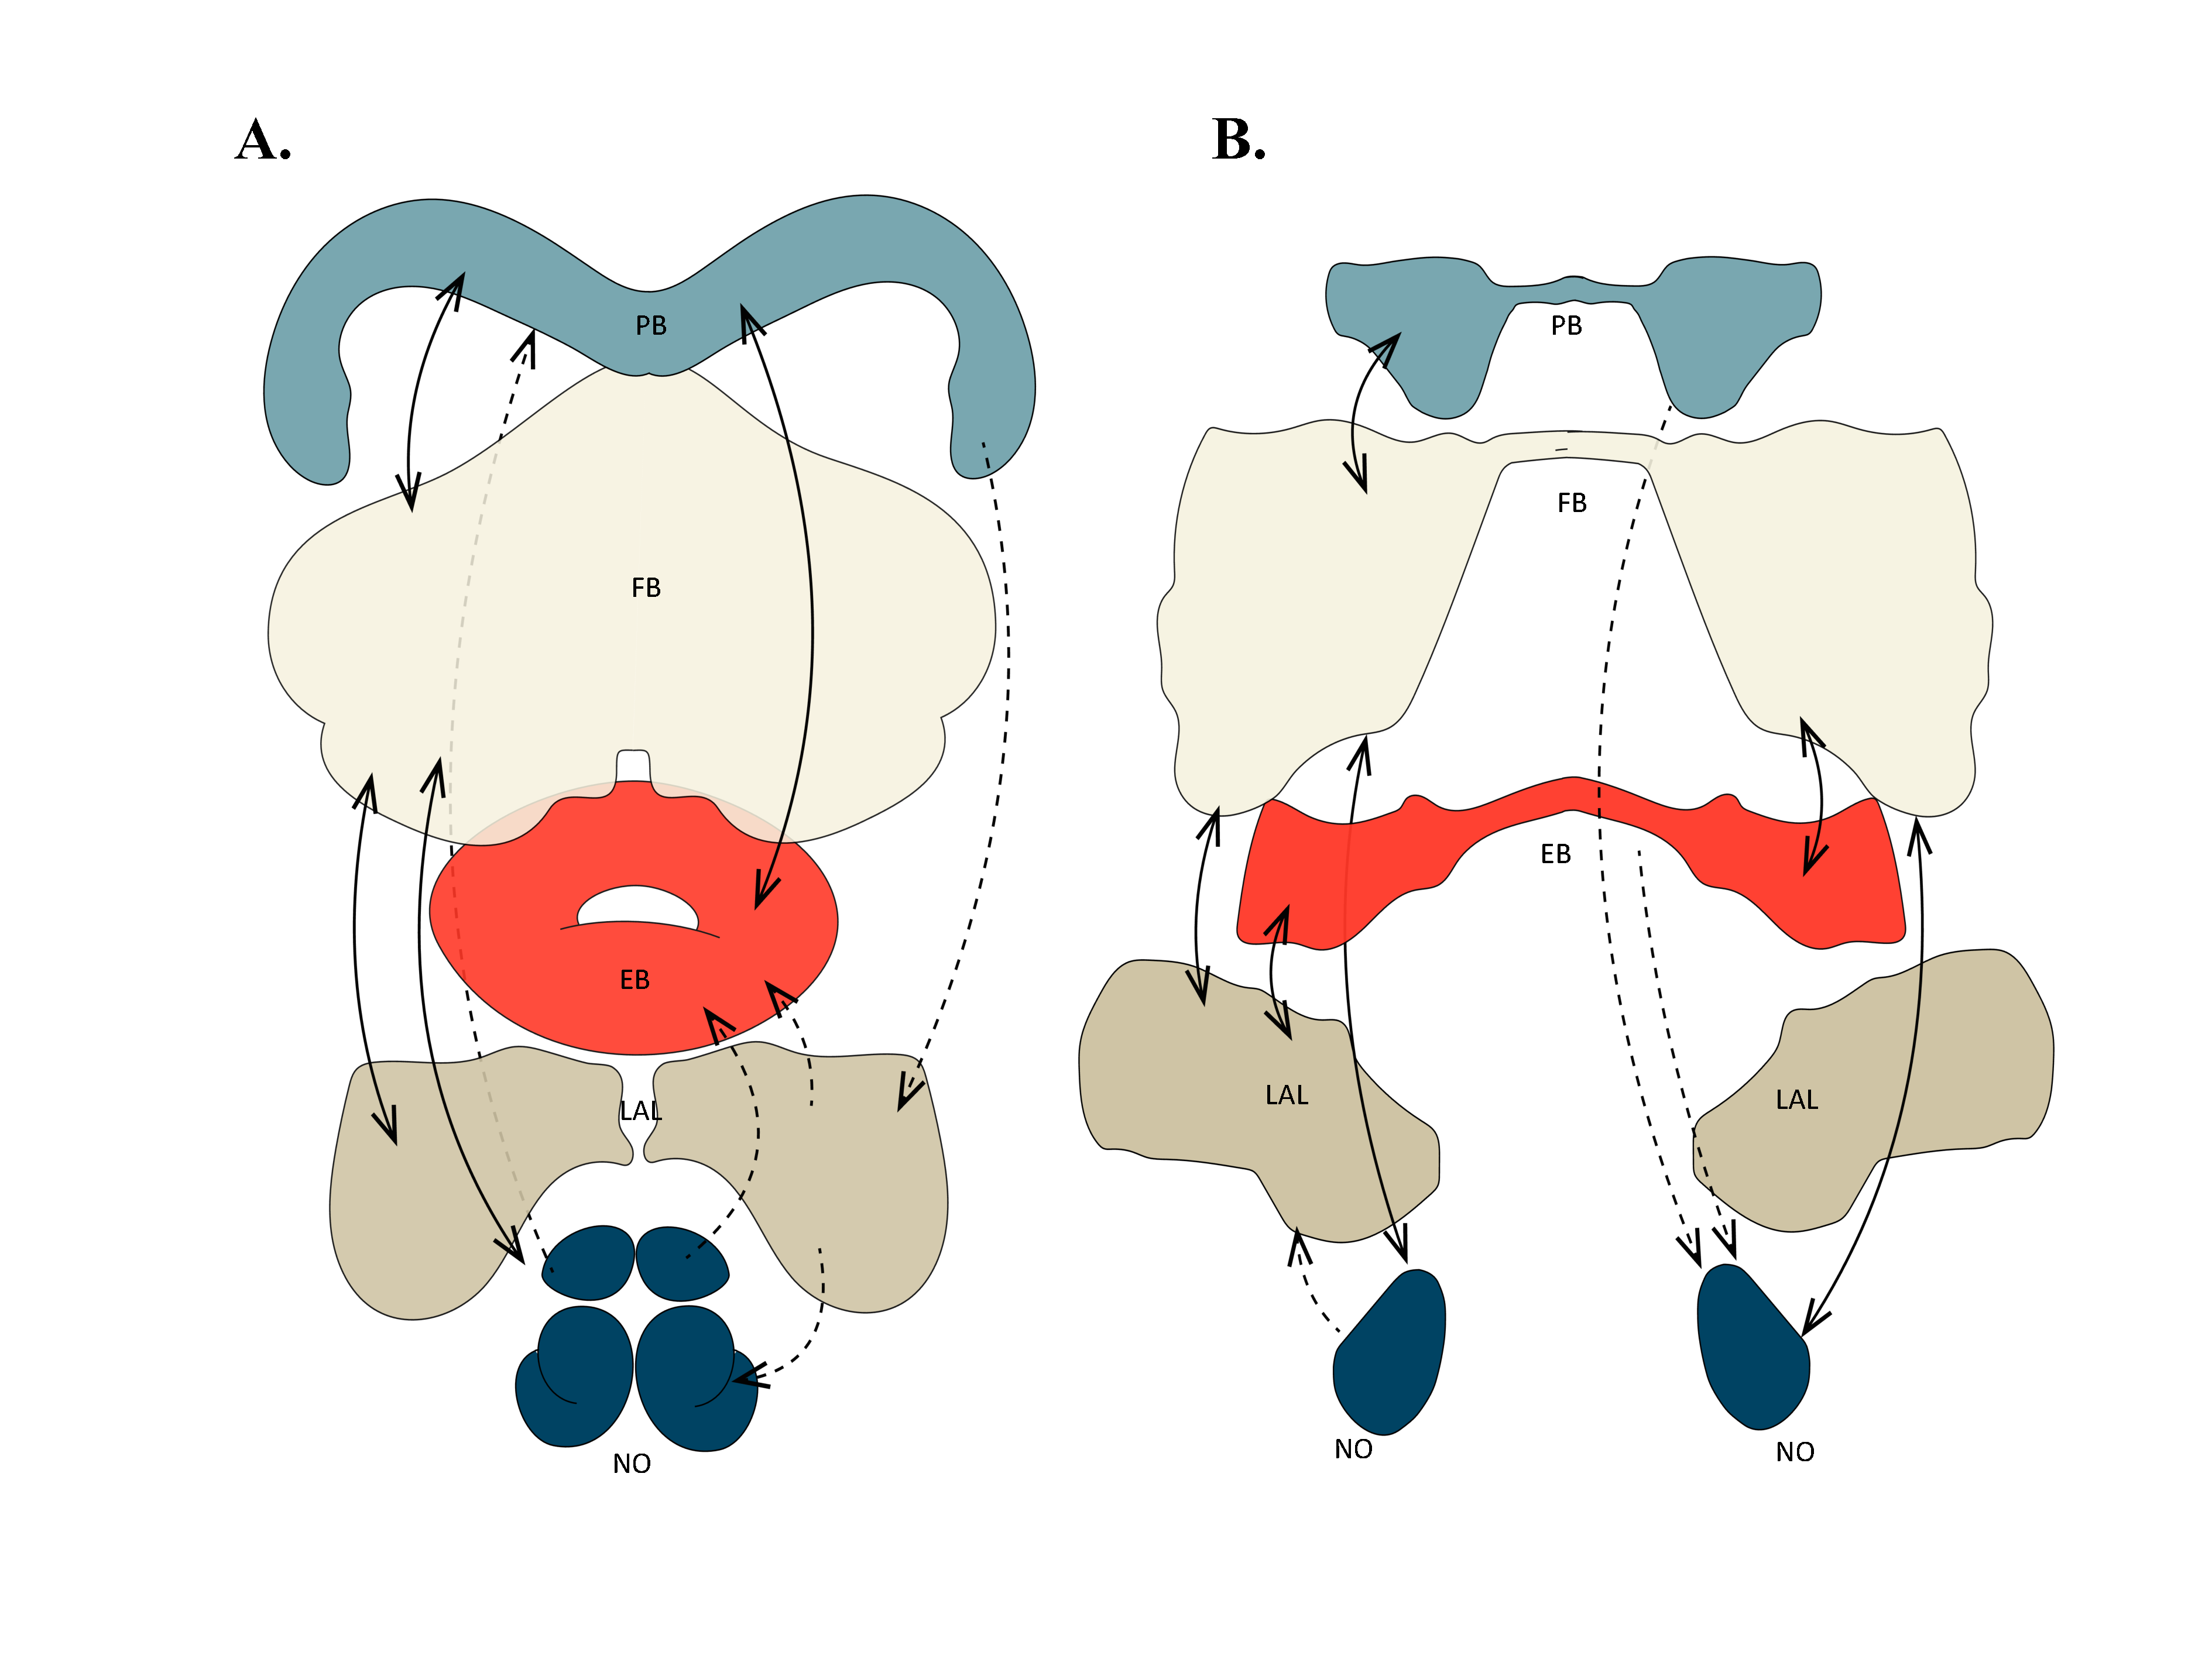
\includegraphics[width=12cm]{/Users/lauralungu/Desktop/Latex/PhD-Thesis/Figs/CX/cxdiagram.pdf}
        \caption[The Central Complex Neuropils in Adult and Larva]{\textbf{The Central Complex Neuropils in Adult and Larva}. Dotted-line arrows represent unidirectional connections, filled-line arrows indicate bidirectional connections. In panel \textbf{A.} we show the adult \textit{\textit{Drosophila}} CX. Bidirectional connectivity is seen between PB-FB, PB-EB, FB-LAL and FB-NO, with unidirectional connections from NO-PB, PB-LAL, LAL-NO and NO-EB; Panel \textbf{B.} displays the larval \textit{Drosophila} CX. Bidirectional connections are  PB-FB, FB-EB, FB-LAL, FB-NO and EB-LAL; unidirectional connections are seen from NO-LAL, PB-NO and EB-NO.The volumes of the adult neuropils were adapted from \citep{franconville2018building}.
        The volumes of the larval neuropils were drawn via CATMAID using the .b and .d parts of the neurons contributing to each.}
        \label{cxdiagram}
    \end{figure}

    \begin{figure}
        \centering
        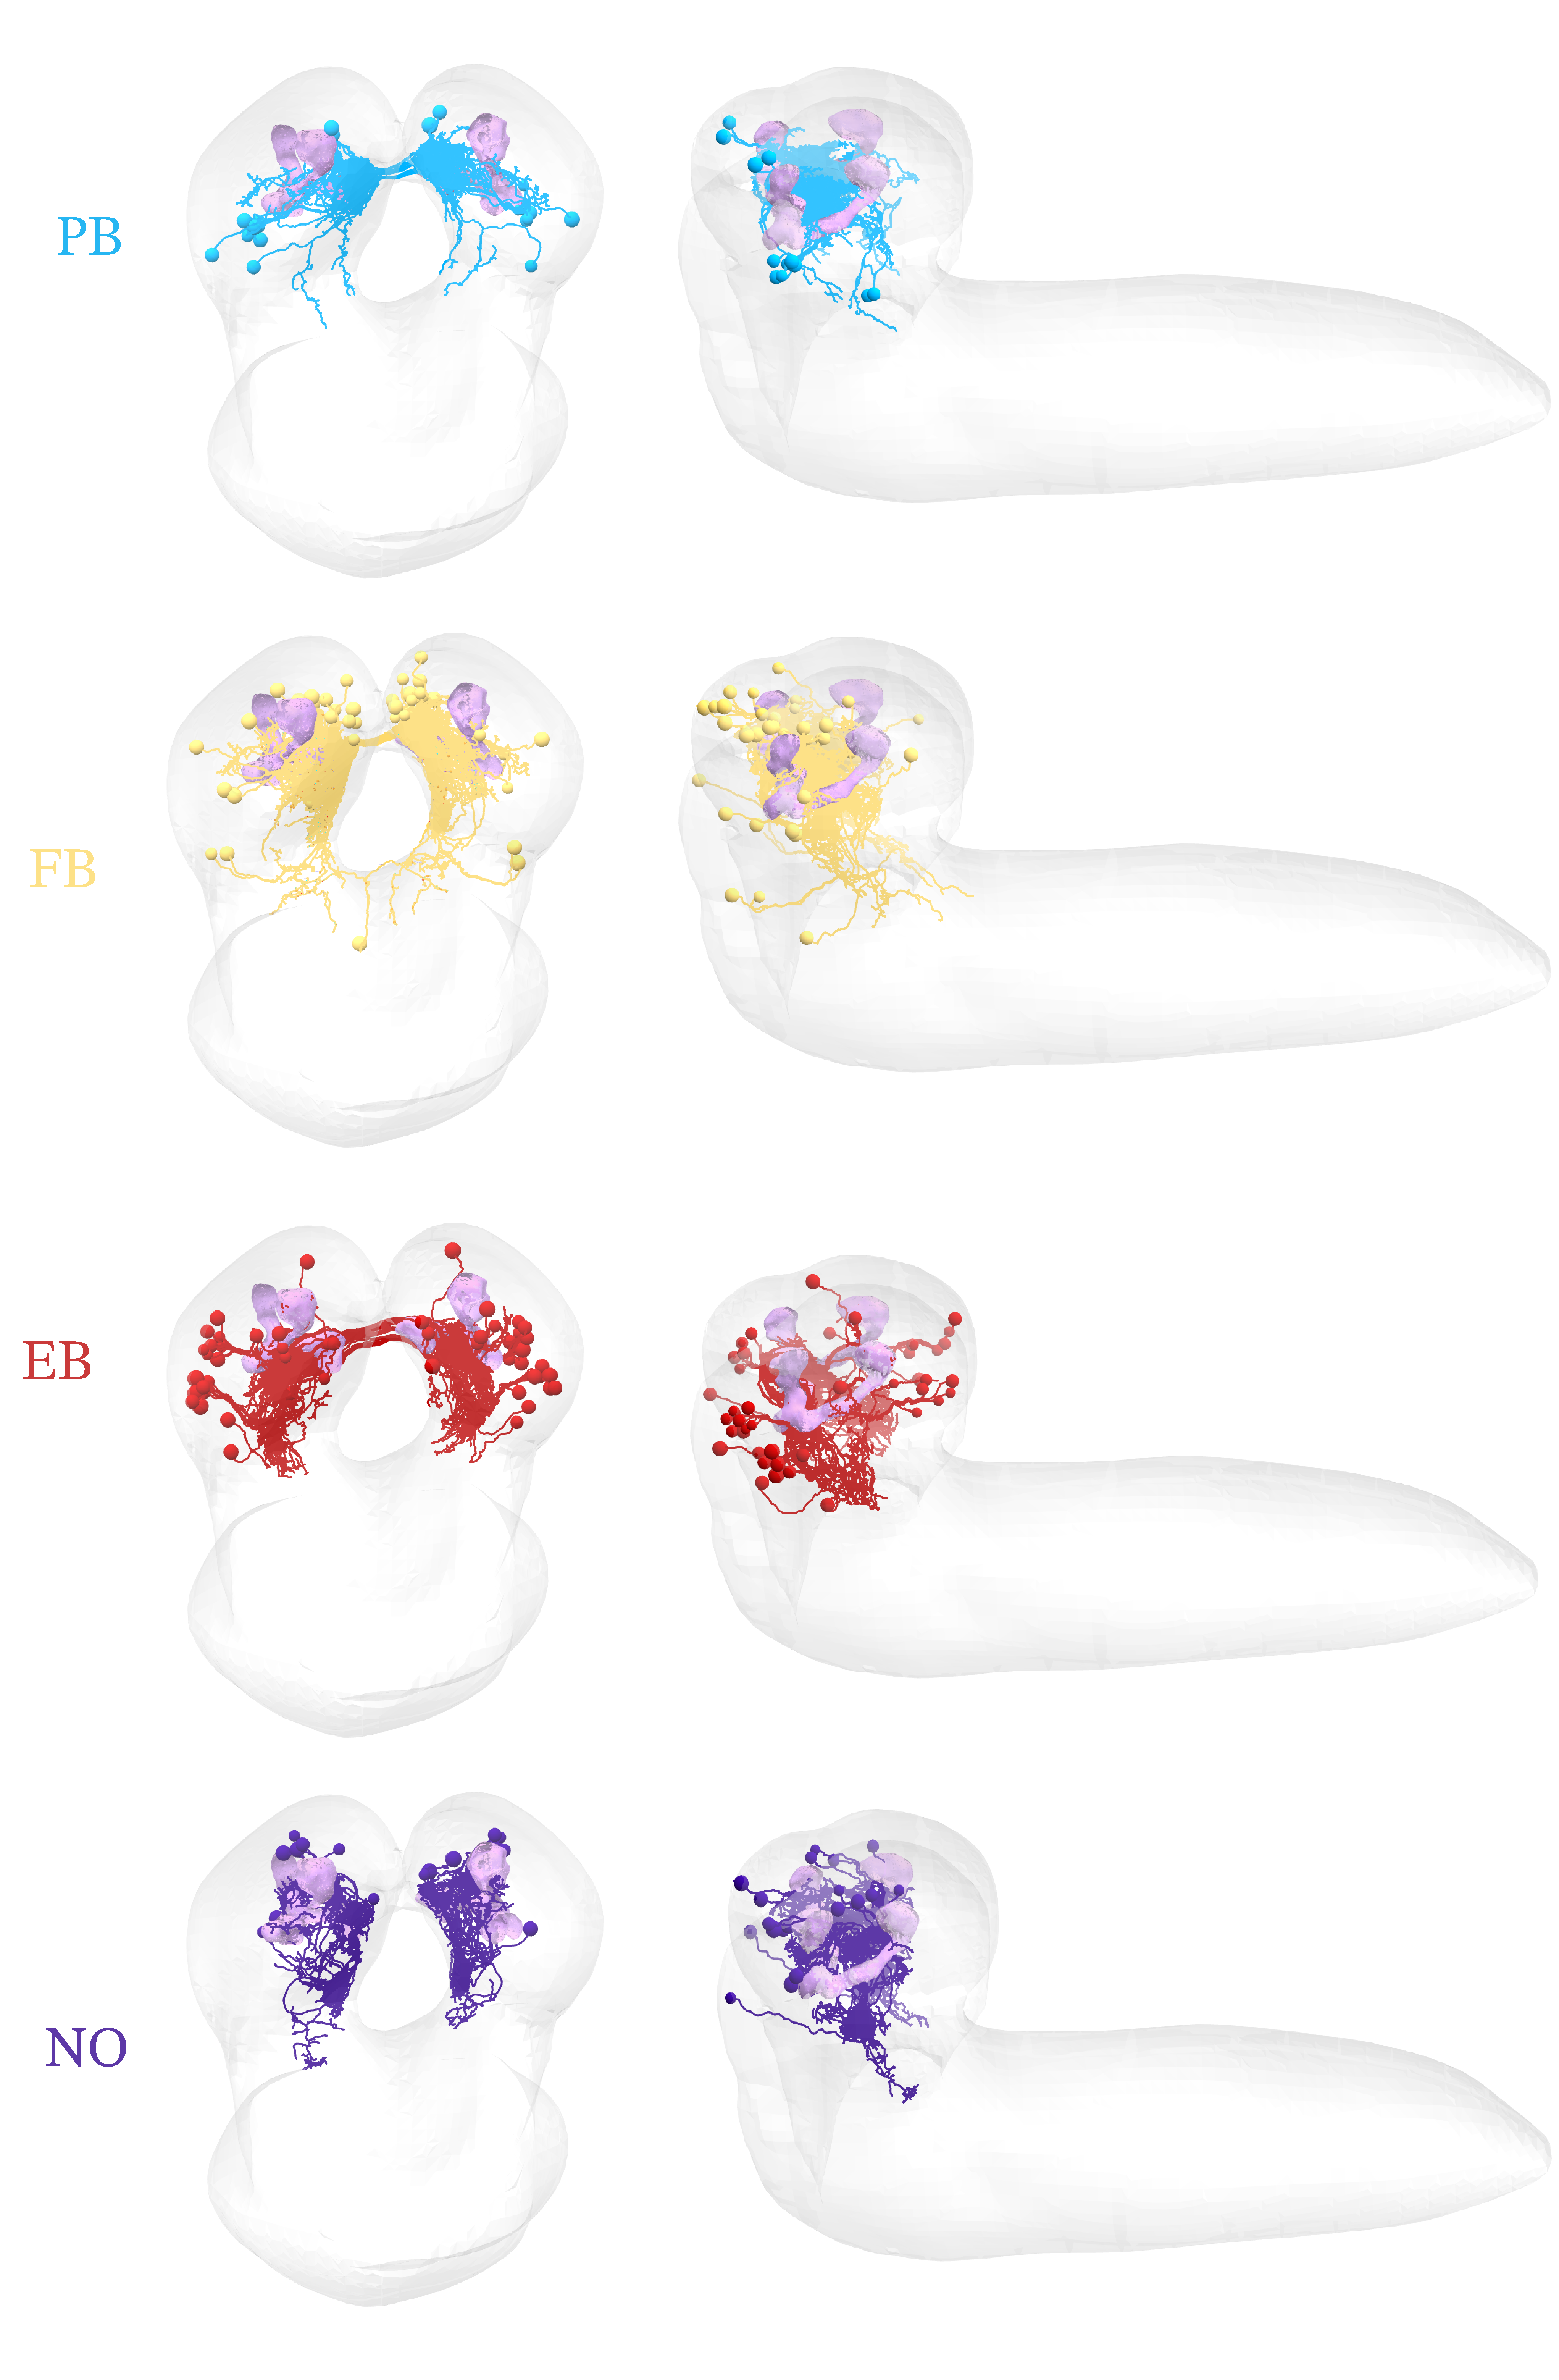
\includegraphics[width=11cm]{/Users/lauralungu/Desktop/Latex/PhD-Thesis/Figs/CX/CATMAIDCXneurons.pdf}
        \caption[Larval CX neuron boutons define the volumes of the 4 main CX neuropils]{\textbf{Larval CX neuron boutons define the volumes of the 4 main CX neuropils.} Posterior and lateral views of neurons that contribute boutons (".b") to each of the 4 neuropils. In concordance with the adult, the PB is the most dorsal and posterior neuropil of the whole brain; the FB occupies an intermediate medial position; the EB is the most medial anterior neuropil (same dorso-ventral level as the mushroom body medial lobe but even more anterior); and the NO are medial and ventral. Note that the white medial space in the larval cartoon is truly devoid of brain tissue: the larval CX neuropils line the medial boundary of the brain hemispheres, with the pharynx occupying most of the intermediate space.
        }
        \label{cxdiagram}
    \end{figure}    

\section{The Central Complex of \textit{Drosophila} Larva}
    \subsection{Protocerebral Bridge}
    \label{PB}
    In searching for the larval PB, we expected two sets of neurons: columnar and horizontal. In larva, four central complex lineages contribute columnar neurons, a subset of which position their dendrites at a posterior-dorsal location. We could not find a central complex lineage that would contribute horizontal fibers at a posterior-dorsal location necessary to intersect and synapse onto the dendrites of the PB columnar neurons; however, we found a larval lineage (DALv1) whose axons are bilateral and project to the appropriate area, and is developmentally related to another central complex lineage (DALv23). This suggests that neurons from non-central complex lineages may be recruited temporarily during the larval period, in a pattern reported so far for the mushroom body (see Discussion; \citep{truman2023metamorphosis}). 

    \textbf{\textit{Larval PB horizontal fibers:}}
    Among neurons of the DALv1 lineage, 4 left-right pairs (named HF-PB for "Horizontal Fiber PB") project their axons bilaterally and across the dendrites of the columnar neurons.
    3 of the 4 pairs present an unusual axon configuration: first, they project contralaterally to drop their first output synapses, with the axon then crossing the midline a second time to return back to the same ipsilaterally corresponding location to again drop presynaptic sites .
    This peculiar axon configuration is unique among all neurons of the entire brain of the larva~(\citep{winding2023connectome}) and suggestive of potentially a delay line for comparing left-right sensory inputs.
    The 4th pair first drops presynaptic sites ipsilaterally and then its axon crosses the midline until reaching the corresponding contralateral location to synapse again~(\ref{DALv1s}). These neurons are PB.b neurons since they contribute axonal butons to the PB. Several of these neurons have their dendrites encolsed in the FB (are FB.d neurons), making them Core CX neurons. 

    \begin{figure}
        \centering
        \includegraphics[width=12cm]{Figs/CX/DALV1s.pdf}
        \caption[PB Dalv1 Neurons]{\textbf{PB Horizontal Fibers (HF-PB).} Two types of horizontal fiber neurons are shown, each with a morphological reconstruction (top) and a simplified schematic (bottom). The mushroom body is shown in magenta. Input synapses (dendrites) are indicated by blue arrows, while output synapses (axons) are indicated by red arrows. Panel \textbf{A.} shows HF-PB1 neurons, characterized by a double-crossing axon; panel \textbf{B.} displays HF-PB2 neurons, with outputs projecting only contralaterally; and panel \textbf{C.} the four bilateral pairs of HF-PB neurons shown together.}
        \label{DALv1s}
    \end{figure}

    % Relative to the root of their dendritic tree, which is ipsilateral, the first set of output synapses are found contralaterally. Then the axon crosses the midline a second time, returning to the ipsilateral hemisphere to establish more output synapses in a spatially symmetric way to the contralateral set of output synapses.

    The presynaptic outputs of DALv1 neurons are symmetric, in that they contact the same homologous pairs of left-right neurons which are predominantly neurons of the columnar system from the DM1-DM4 lineages.%figure with columnar and horizontal connections


    \begin{table}[h!]
    \centering
    \begin{tabular}{l|cccccccccc}
    \toprule
    \textbf{PB Horizontal} & \multicolumn{10}{c}{\textbf{PB Columnar}} \\
    \cmidrule(lr){2-11}
    & \rot{PB to NO,\\MB2ON-204\\\_l}
    & \rot{PB to NO,\\MB2ON-204\\\_r}
    & \rot{PB to NO,\\MB2ON-241\\\_r}
    & \rot{PB to NO,\\MB2ON-241\\\_l}
    & \rot{PB to EB,\\MB2IN-195\\\_l}
    & \rot{PB to EB,\\MB2IN-195\\\_r}
    & \rot{PB Descending\\\_1\_l}
    & \rot{PB Descending\\\_1\_r}
    & \rot{PB Descending\\\_2\_l}
    & \rot{PB Descending\\\_2\_r} \\
    \midrule
    HF-PB1\_r
    &  &  &  &
    & \cellcolor{forest1}1
    & \cellcolor{forest3}13
    & \cellcolor{forest3}15
    & \cellcolor{forest4}22
    & \cellcolor{forest5}26
    &  \\

    HF-PB1\_l
    &  &  &  &
    & \cellcolor{forest1}1
    & \cellcolor{forest2}11
    & \cellcolor{forest2}9
    & \cellcolor{forest4}23
    & \cellcolor{forest5}27
    &  \\

    HF-PB3\_r
    & \cellcolor{forest3}12
    & \cellcolor{forest4}21
    & \cellcolor{forest3}17
    &
    & \cellcolor{forest2}8
    & \cellcolor{forest2}10
    & \cellcolor{forest2}9
    & \cellcolor{forest3}13
    & \cellcolor{forest3}13
    & \cellcolor{forest4}18 \\

    HF-PB3\_l
    & \cellcolor{forest3}17
    & \cellcolor{forest4}22
    & \cellcolor{forest2}7
    &
    & \cellcolor{forest2}8
    & \cellcolor{forest3}11
    & \cellcolor{forest3}14
    & \cellcolor{forest2}10
    & \cellcolor{forest3}13
    & \cellcolor{forest4}19 \\
    \bottomrule
    \end{tabular}
    \caption[PB horizontal fibers connection to  PB columnar ]{}
    \label{PBconnections}
    \end{table}


    The axons of these 4 pairs of HF-PB neurons are tiled dorso-ventrally, falling into two bilaterally symmetric groups which we interpret as defining 2 + 2 bilaterally arranged PB compartments, each innervated by 2 pairs of axons (Figure \ref{DALv1s}C). %potentially different figure see TODO list 


    The dendrites of these 4 pairs of DALv1 neurons (HF-PB) are ipsilateral and dorsal, receiving polysynaptic inputs from vision and olfaction, like in the adult PB~(\citep{hulse2021connectome}). In the larva, we found that these multi-sensory inputs to the horizontal fibers of the PB are mediated by Convergence Neurons (CN-53 and CN-54, among others; \citep{eschbach2021circuits}) that, as their name indicates, integrate inputs from both Mushroom Body Output Neurons (MBONs) and from the Lateral Horn (LH) such as olfactory and visual PNs \citep{eschbach2020recurrent}). This circuit architecture indicates that sensory inputs arriving to the larval PB will have been modulated or gated by previously established associative memories, with implications for spatial navigation.

    Three more larval lineages contribute HF-PB neurons: the BLAvm (neuron SLR), the BLAd-OL (neuron MB2ON-63), and the DPMm2 (neuron ADC1),  with one pair of neurons each. 

    MB2ON-63 presents a bilateral axon similar to the 4th pair of HF-PB (DALv1), and an ipsilateral dendrite that integrates inputs from multiple convergence neurons (CN-54, CN-9), MBONs (MBON-c1, MBON-d1), and sensory PNs (olfactory mPN B1, visual PVL09).

    SLR presents a contralateral axon that spans both the FB and PB, and an ipsilateral dendrite that integrates inputs from MB2ON-63, CN-9, and the FB intrinsic neuron MB2ON-175 (see below), in addition to a long tail of weaker input from ascending neurons relaying information from the somatosensory system.

    ADC1 presents an ipsilateral dendrite projecting to the posterior brain and a bilateral axon circumscribed to the PB. These neurons integrate inputs from multiple sensory PNs (mPN B2, mPN 5 (also known as mPN BAmd1-g), mPN A1, and weakly from others), a convergent neuron (CN-35), MB2ON-94, and a few others weakly. Their axons target primarily HF-PB neurons (DALv1), but also convergent neurons strongly (CN-56, CN-15, CN-35).


    % check for more CNs or other neurons converging onto PB DALv1 dendrites
    %ANSWER: CN35, CN45, CN9 low syn count CN26, CN15
    %as well as from other sensory modalities (Table \ref{sensoryinputs})
    %TODO: describe dendritic and axonic contributions in specific (especially from AL, OL and MB) 
    %2 systems: pattern of input of dendrites of the DALv1 s.
    % MB2ON-175 & 48 & 208 
    % given the PB1-4 compartments, which ones are connected to the MBONs, and the CNs. 175 targets one compartment, 208 targets another.  The pattern is that CNs connect to one compartment of the PB while simultaneously connecting to another CN that connects to the opposite compartment - there could be a gating mechanism. 
    %MB2ON 202 - feedback from the NO to the PB dalv1 

    \textbf{\textit{Larval PB columnar neurons:}}

    In the larva, the columnar system consists of neurons from 4 central complex lineages (DPMpm1, DPMpm2, DPMm1 and CM4) that also generate the columnar neurons of the adult (DM1, DM2, DM3 and DM4, correspondingly: these are the same lineages with different names for the larva and the adult for historical reasons).
    Larval columnar neurons present small, narrow dendrites circumscribed within the 2 + 2 compartments defined by the axons of the HF-PB (DALv1) neurons, from whom they recieve synapses. These are catalogued as PB.d neurons since they contribute their dendrites to the PB.

        \begin{figure}
            \centering
            \includegraphics[width=12cm]{Figs/CX/PBcolumnar.pdf}
            \caption[PB columnar neurons]{\textbf{PB columnar neurons.} The three types of columnar neurons are shown. The mushroom body is shown in magenta. \textbf{A.} Neurons projecting from the PB to the NO (PB.d NO.b), with the NO neuropil shown in dark blue. \textbf{B.} Neurons projecting from the PB to the EB (PB.d EB.b), with the EB represented by the red structure beneath the mushroom body. \textbf{C.} Descending PB neurons projecting toward the SEZ or the VNC.}
            \label{pbcolumnar}
        \end{figure}

    Among the columnar neurons, a subset project their axons directly to the NO (Fig. \ref{pbcolumnar}A), and another subset project directly to the larval EB (Fig. \ref{pbcolumnar}B).

    We did not find among the larval columnar neurons any whose axon would project to more than one CX neuropil, despite such types being common in the adult~\citep{wolff2015neuroarchitecture, wolff2018neuroarchitecture, hulse2021connectome}.
    Beyond the canonical columnar neurons projecting to other CX neuropils, we found some whose axons descend directly to the SEZ or nerve cord~(Fig. \ref{pbcolumnar}C).


    % TODO Discussion point: this is different than in the adult. 
    % QUESTION: in the adult, are there columnar neurons that descend to the nerve cord? We have them too in larvae. Should mention them.
    %ANSWER: see figure 63A Hulse et al. supplement 1 PFL -> MDNs (I have a feeling mdn is smth else in adult)
    %In the \textit{Drosophila} larva Electron Microscopy (EM) volume, we found a putative PB situated at the most medial-posterior side of the brain, that receives high levels of visual input and is made of neurons belonging to lineages DM2 (DPMpm1 in the larva) and 8 columnar neurons(4 pairs) belonging to the lineage DALv1. 
    % also - a dopaminergic pathway formed by large field CIVP neurons that relay IDFP signals to the entire PB



    \subsection{Ellipsoid Body}
    %In the 1st instar larva, we found a group of 8 pairs of reciprocally connected neurons from lineage DALcl12 known to produce wedge-neurons in the adult, and categorised these together with one other pair of lineage Dalv23 (which produces ring neurons in adult) with the same connectivity pattern as wedge-neurons. Both their dendrites and axons are very small, and tiled medio-laterally, defining 8 compartments with one single neuron pair contributing to each. These are the intrinsic set of neurons, fully enclosed within the putative larval EB. Similarly, we found one pair of neurons of the BAmv1/2 lineage - known to contribute to ring neurons in adult flies - that receive visual input via PB neurons, and reciprocally interconnects with the previously mentioned wedge-neurons, and whose axons are fully contained within the space defined by the wedge neurons. We categorised these as larval "ring" neurons.

    
    \textbf{\textit{Larval EB Wedge neurons:}}
    In the larval brain, we found a group of 8 pairs of reciprocally synaptically connected neurons from larval lineage DALcl12, known to produce Wedge neurons in the adult, so we named them Wedge neurons.
    Both their dendrites and axons are very small, and tiled medio-laterally, defining 8 compartments with one single neuron pair contributing to each (Fig. \ref{EBneurons}C).
    We found an additional pair of neurons from larval lineage DALv23 (which produces ring neurons in the adult) with the same connectivity pattern as Wedge neurons (Fig. \ref{EBneurons}B). All wedge neurons have contribute both axons and dendrites to the EB,making them EB.d.b neurons, and Core CX neurons, accordingly.

    While Wedge neurons make both axo-dendritic and axo-axonic synapses onto each other (like the AL Picky LNs do; \citep{berck2016wiring}), their dendrites integrate inputs from a variety of sources, including MBONs (MBON-e1, MBON-e2, MBON-g1, MBON-g2, MBON-b3, MBON-m1, and weak inputs from more), convergence neurons (CN-14, CN-25, CN-62, CN-38), and MB feedback neurons (FBN-13, FBN-19, FBN-21), indicating that the EB is intimately and intricately involved with the MB (see below).
    Wedge neurons, like the adult, receive further axo-axonic synapses from Ring neurons (see below; RN1/2, also known as FBN-20; and RN3).
     

        \begin{figure}
            \centering
            \includegraphics[width=12cm]{Figs/CX/EBneurons.pdf}
            \caption{\textbf{Ellipsoid Body Neurons} Ring and Wedge Neurons with their corresponding lineages. The mushroom body is shown in magenta as a landmark in the larval brain. \textbf{A.} Ring neurons of lineage Dalv23, namely RN1/2a and RN1/2b; \textbf{B.} Ring neuron RN3 originating from lineage BAmv1/2; and \textbf{C.} The 8 EB wedge neurons (W1-8) originating from DALcl12 lineage. Panel \textbf{D.} depicts all these neurons stacked together to form the EB}
            \label{EBneurons}
        \end{figure}

        \begin{figure}
            \centering
            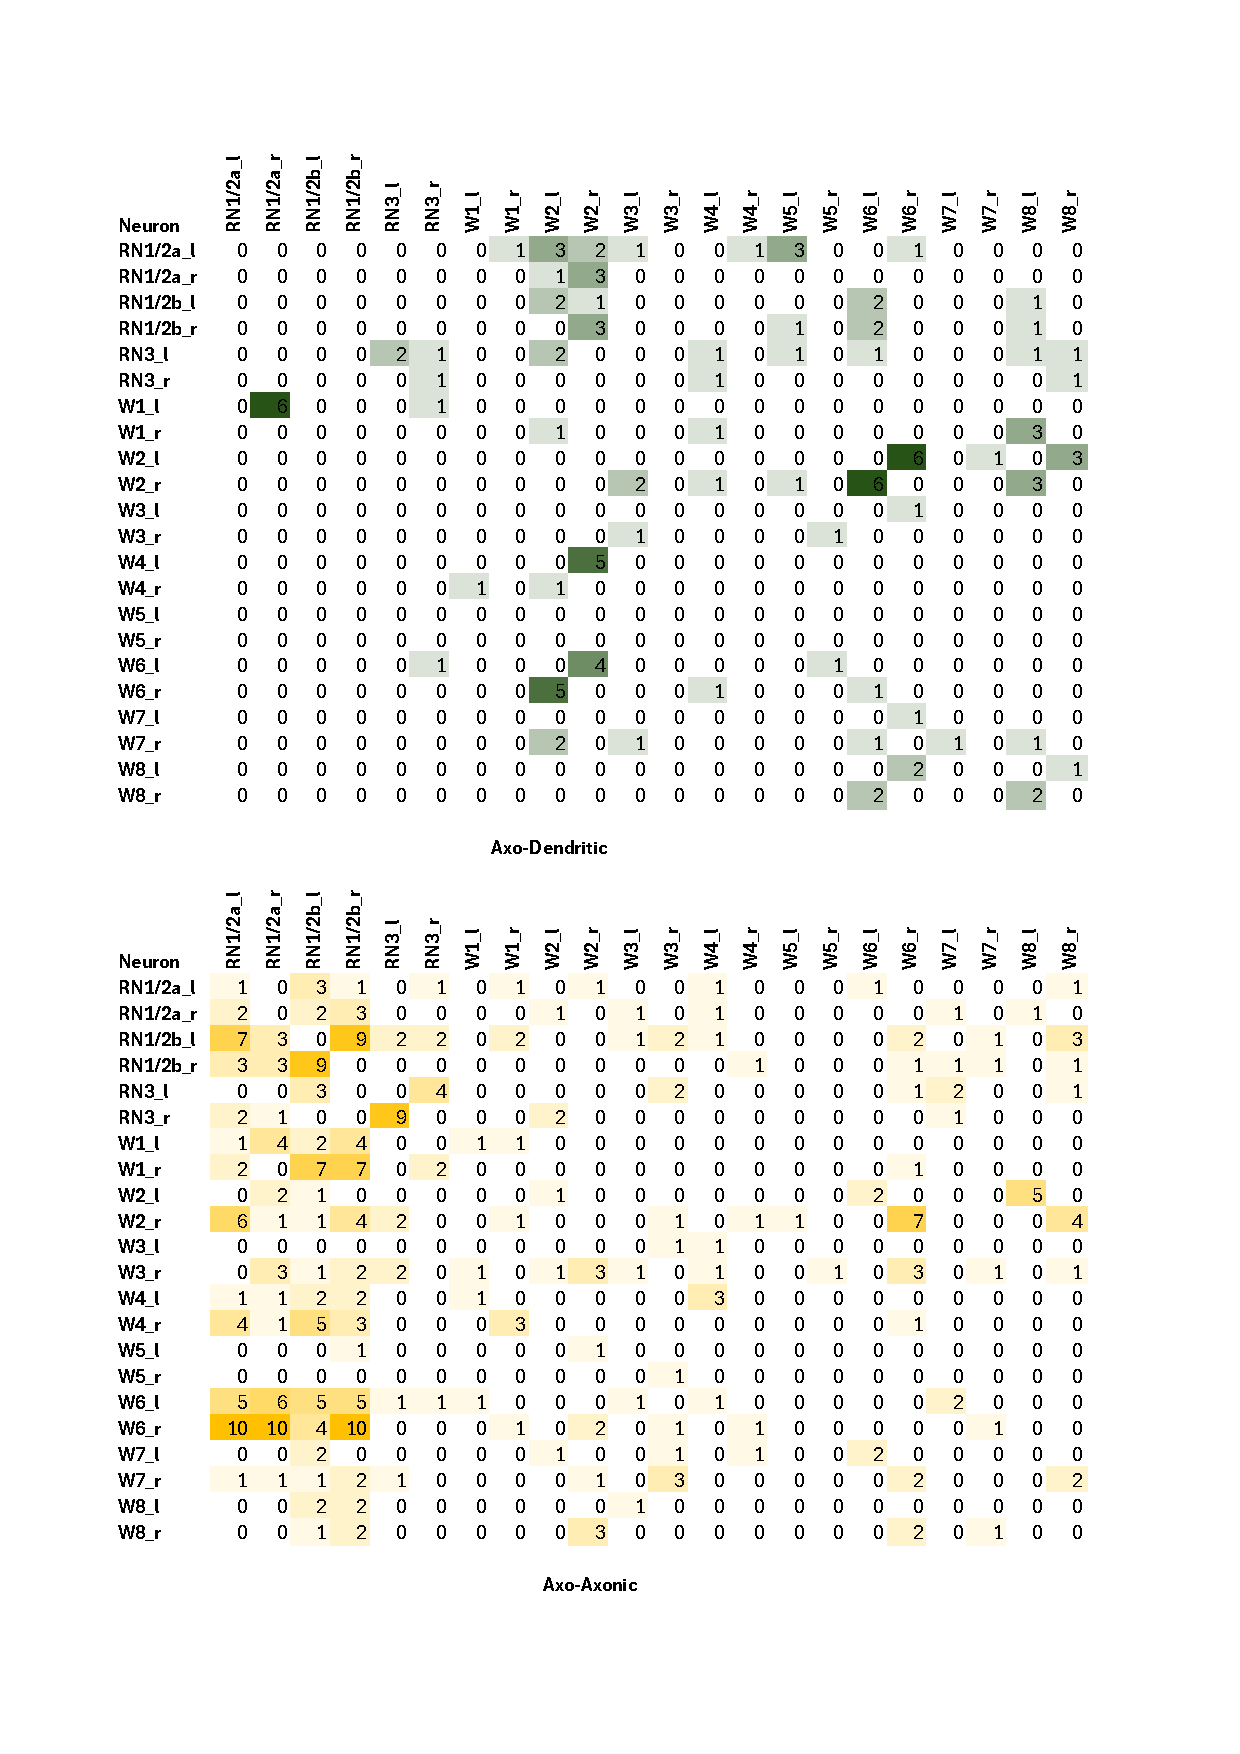
\includegraphics[width=12cm]{Figs/CX/EBneuronsmatrix.pdf}
            \caption{\textbf{EB Neurons Connectivity.} Both tables display the connectivity patterns among ring and wedge neurons in the ellipsoid body (EB). Each neuron is separated into left (\_l) and right (\_r) counterparts to represent lateralization. \textbf{Upper table:} axo-dendritic connections (color-coded in the green spectrum). \textbf{Lower table:} axo-axonic connections (color-coded in the yellow spectrum).}
            \label{EBmatrix}
        \end{figure}



    \textbf{\textit{Larval EB Ring neurons:}}

    We found one pair of neurons (RN3) of the larval BAmv1/2 lineage (corresponding to adult lineage LALv1 known to generate ring neurons) that receive visual input via PB columnar neurons, and reciprocally synapses axo-axonically with larval Wedge-neurons (Fig. \ref{EBneurons}A).
    Their axons are fully contained within the space defined by the wedge neurons.
    Similarly, we found two pairs of neurons (RN1/2) from the larval DALv23 lineage (adult EBa1 lineage, also known to generate ring neurons), synaptically connected like RN1/2 (Fig. \ref{EBneurons}B). We classified all of these as larval EB Ring neurons, all of them having both dendrites and axons inside the EB, making them EB.d.b neurons, and as such, Core CX neurons. 

    \textbf{\textit{Additional EB.d Neurons}}
    There are seven more pairs of EB.d (neurons that contribute presynaptic sites to the EB) that didn't fall under ring or wedge neuron categories. Two of these are MB Dopaminergic neurons (DAN-d1 and DAN-g1), another 3 are LAL intrinsic neurons, and the last 2 are MB second order output neurons. %TODO add appendix 


    \textbf{\textit{Sensory inputs to the larval EB:}}

        \begin{figure}
            \centering
            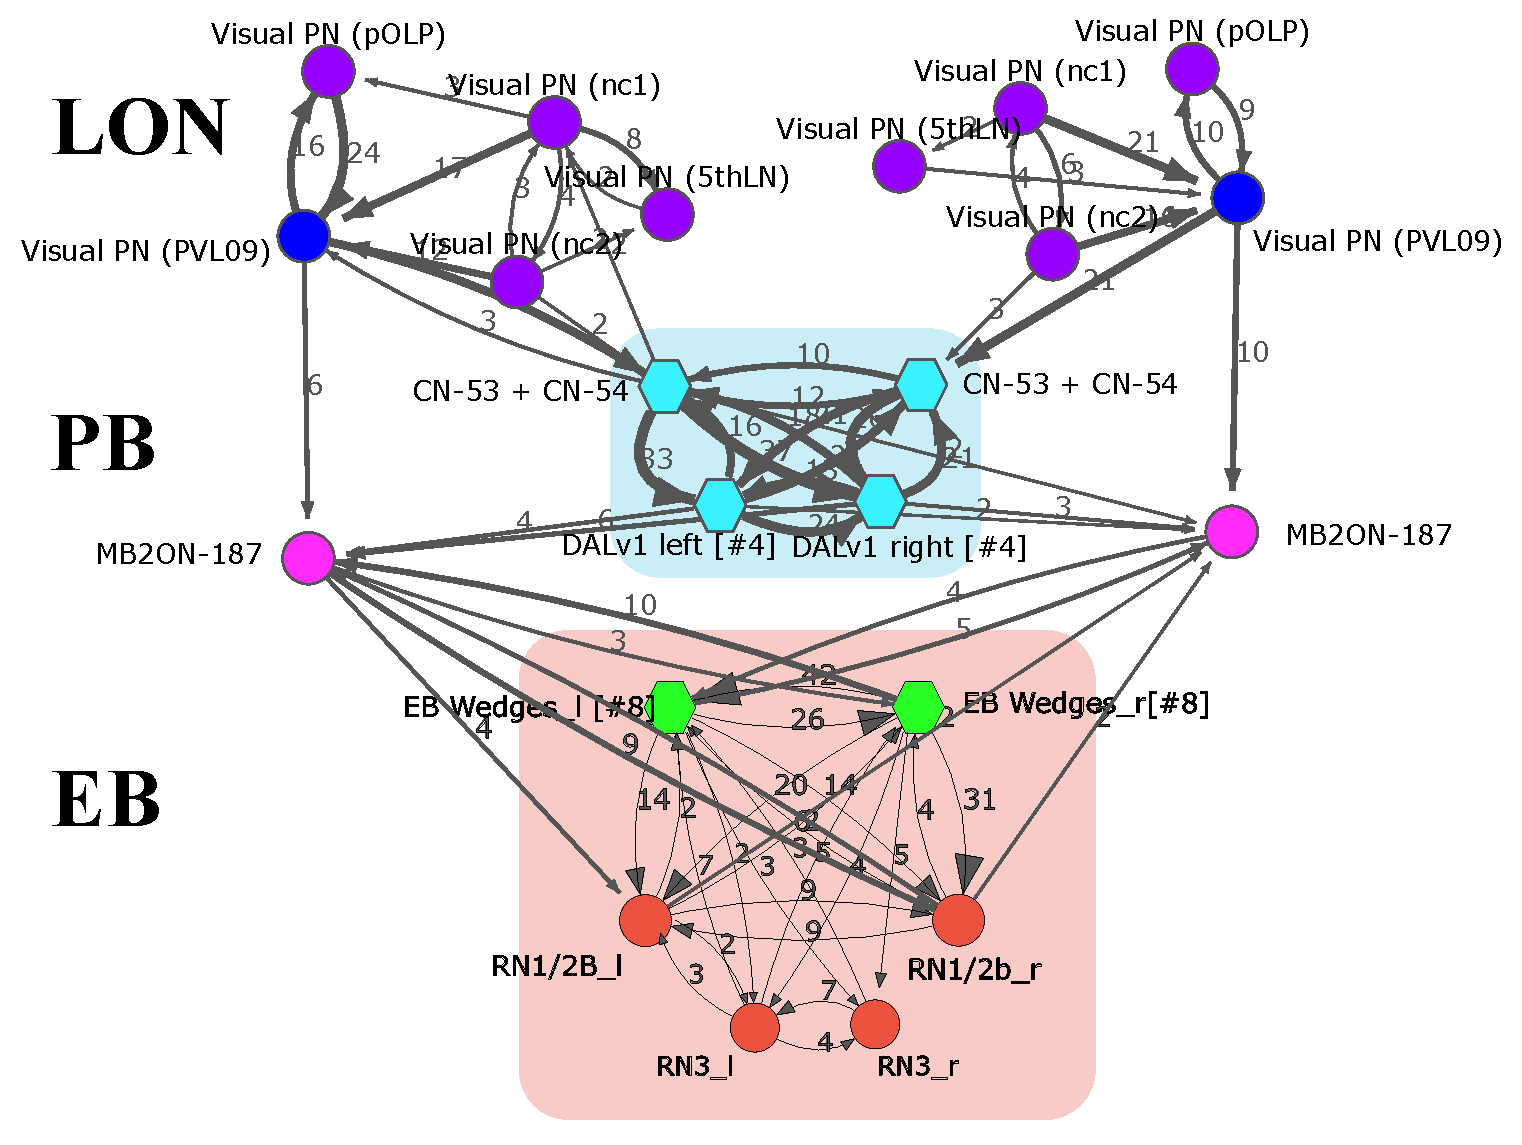
\includegraphics[width=10cm]{Figs/CX/visualPNstoPBEB.pdf}
            \caption{\textbf{Visual Input into the EB}. Input from visual Projection Neurons (Visual PN) to the Ellipsoid Body~(EB) via two convergence neurons~(CN53, CN54), a pair of PB DALv1s and a second-order Mushroom Body output neuron~(MB2ON-187).}
            \label{visualPBEB}
        \end{figure}
        
    % Blue photoreceptors -> Visual PN (PVL09) -> MB2ON-187 (TuBu?) -> EBa1 ring neurons (DALv23)
    In the adult, the EB is known to receive visual inputs via a polysynaptic pathway (see Fig. 6 in \citep{hulse2021connectome}, and Fig. 4 in \citep{omoto2018neuronal}).
    In the larva, we find that the main visual PN for negative phototaxis, PVL09 \citep{Humberg2018PVL09}, synapses axo-dendritically onto MB2ON-187, which relays sensory inputs from visual and other sensory modalities axo-axonically onto larval Wedge neurons and Ring neurons (Fig. \ref{visualPBEB}).
    MB2ON-187 is named so for being postsynaptic to MBONs (MBON-c1 in particular; \citep{eschbach2021circuits}).
    Through MB2ON-187, multiple sensory PNs (PVL09, mgPN 7) and many neurons postsynaptic to MBONs (MB2ONs) synapse onto Wedge neurons (see Suppl. Connectivity Matrix).
    The latter indicate, again, that MBONs modulate or filter sensory inputs converging onto the EB.



    \subsection{Fan-Shaped Body}

    In the larva, we found a number of putative FB horizontal/tangential cells
    originating in lineages known to contribute neurons to the adult FB. Characteristically, most present a bilateral axon closely wrapping around the midline, and an ipsilateral dendrite positioned within the superior dorsal protocerebrum (dorsal anterior neuropil) where they integrate numerous inputs from MBON axons. Among the various neurons with dendrites within this very medial neuropil, we find neurons from lineages known to contribute to the adult FB and whose axons project to the putative larval NO, EB, PB and LAL.


    \textbf{\textit{Larval FB tangential cells}}

    % TODO: FB.b neurons
    % Types:
    % 2. CX columnar FB.b PB.b (and the dendrites?). Some are postsynaptic to Munin (feeding system, Schlegel et al. 2016 eLife)
    % 3. CX columnar FB.b (and the dendrites?)
    % 4. MB2ON-208 FB.b
    % 5. SEZ FB.b
    % 6. VNC pCC FB.b (insulin?)
    % 7. rest of the brain FB.b

    We found a diverse and large collection of larval FB tangential cell types.
    All types contribute synapses rather specifically to the FB and are hence labeled as FB.b, a defining feature across them all.
    The somas originate in a number of larval lineages whose adult homologs are known to contribute neurons to the adult FB (see above), but also a few from the nerve cord, projecting their ascending axons directly to the FB such as the pCC neurons (a cell type first reported in grasshopper \citep{goodman1984pCC} and later in the \textit{Drosophila} embryo \citep{jacobs1989pCC}). The axons of the pCC project to the ipsilateral FB. The set of ascending neurons isn't complete, for the ventral nerve cord (VNC) remains incompletely mapped.

    Among all neurons projecting their axons to the FB, many are brain neurons that do so with a typical bilateral horseshoe ('hs') axon, and hence we named then hs-FB, with a numeric label for each subtype.

        \begin{figure}
            \centering
            \includegraphics[width=10cm]{Figs/CX/HS-FBneurons.pdf}
            \caption{\textbf{FB tangential cells,} also known informally as "horseshoe" neurons for the shape of their bilateral axons. The seven hs-FB subtypes are shown, each with a morphological reconstruction (top) and a simplified schematic (bottom). Input synapses (dendrites) are indicated by blue arrows, and output synapses (axons) by red arrows. The mushroom body is shown in magenta. Neuron counts (left+right) are given below each schematic. \textbf{A–C.} Individual examples of hs-FB.1, hs-FB.2, and hs-FB.3. \textbf{D.} Overlay of hs-FB.1 through .3, illustrating the FB compartments they define. \textbf{E–H.} Individual examples of hs-FB.4 through .7.}
        \label{fig:HSFBneurons}
        \end{figure}

    The DM1-DM4 lineages that contribute to the adult CX also generate a number of neurons in the larva (larval lineages DPMm1, DPMpm1, DPMpm2, and CM4-vm, respectively). Targeting the FB, there are several major subtypes. First, 6 pairs of neurons (hs-FB.1) with a bilaterally symmetric axon that tightly lines the medial surface in a horseshoe shape, and with a smallish dendrite dorsal and slightly lateral to the FB, within the medial side of the superior protocerebrum. Second, 2 pairs of neurons (hs-FB.2) also with bilaterally symmetric axons but that target the more posterior-lateral FB and beyond into the larval PB,
    with also ipsilateral dendrites that extend anteriorly and ventrally along the neuraxis.
    Third, a pair of neurons (hs-FB.3) with bilateral axons placed towards the most posterior end of the FB and perhaps beyond, into the lateral side, and with small ipsilateral dendrites.
    The axons of all 6 pairs of hs-FB.1 neurons define the ventral layer of the FB, and the axons of the hs-FB.2 the dorsal one, which is shorter and more anterior. The hs-FB.3 axons project in between the other two types but also cover the posterior-dorsal area that hs-FB.2 doesn't (Fig. \ref{fig:HSFBneurons}). 
    The larval BAla34 lineage generates sensory PNs, of which two pairs (hs-FB.4) present the typical bilateral axon and their dendrites collect inputs from the ventral posterior brain where ascending PNs from the somatosensory system (mostly mechanosensory) project their axons. One of the pairs is also NO.d (collects inputs from NO.b neurons).
    The larval BAmd2 lineage contributes two pairs of neurons (hs-FB.5) with a bilateral axon and dendrites that cover a region medial but lateral to the FB, and also far more ventral.
    The larval DALl1 lineage contributes two pairs of neurons (hs-FB.6) with a bilateral axon and dendrites integrating inputs from the intermediate and lateral areas to the FB, primarily from neurons postsynaptic to ascending mechanoreceptive neurons like A00c \citep{ohyama2015multilevel}. A number of neurons presynaptic to hs-FB.6 are also labeled as FFNs and MB2INs, meaning they converge onto MB DANs, MBINs and OANs \citep{eschbach2020recurrent}.
    The larval CPa lineage contributes a pair of neurons (hs-FB.7) with a bilateral axon and dendrites that cover the most posterior end of the FB, or right outside, plus sparsely a space lateral to the FB, collecting inputs from polysynaptic pathways originating in somatosensory mechanoreceptive neurons.


    %%%Other FB.b neurons 
    Finally, the DPLal1-3 lineage contributes a pair of small neurons (ip-FB.1) with an ipsilateral-only axon targeting the most posterior lateral side of the larval FB, and with dendrites more lateral that integrate inputs from a variety of neurons, some of which are NO.d.

     

    \textbf{\textit{Larval FB columnar neurons}}

    % TODO: FB.d neurons
    % Types:
    % 1. FB.d HF-PB (DALv1; which are also MB2ONs)  !!!
    % 2. FB.d NO.b MB2ON-201, MB2ON-204, CN-34
    % 3. FB.d FFN-6  -> upstream of MB DANs
    % 4. FB.d ni (MB non-intrinsic early-born KC-like but not KCs), two cell types
    % 4b. FB.d PB.d ni
    % 5. FB.d "descending contralateral 2"
    % 6. FB.d horseshoe that aren't FB.b
    % 7. FB.d FB-NO 1
    % 8. FB.d NO.d " CM4 cen ant 1" (and the axons?)

    % TODO Note the loop between FB and NO, with NO.d-FB.b and FB.d-NO.b neurons.

    By definition, all larval FB columnar neurons present dendrites in the FB (are FB.d), and are postsynaptic to FB.b neurons.

    \begin{figure}
        \centering
        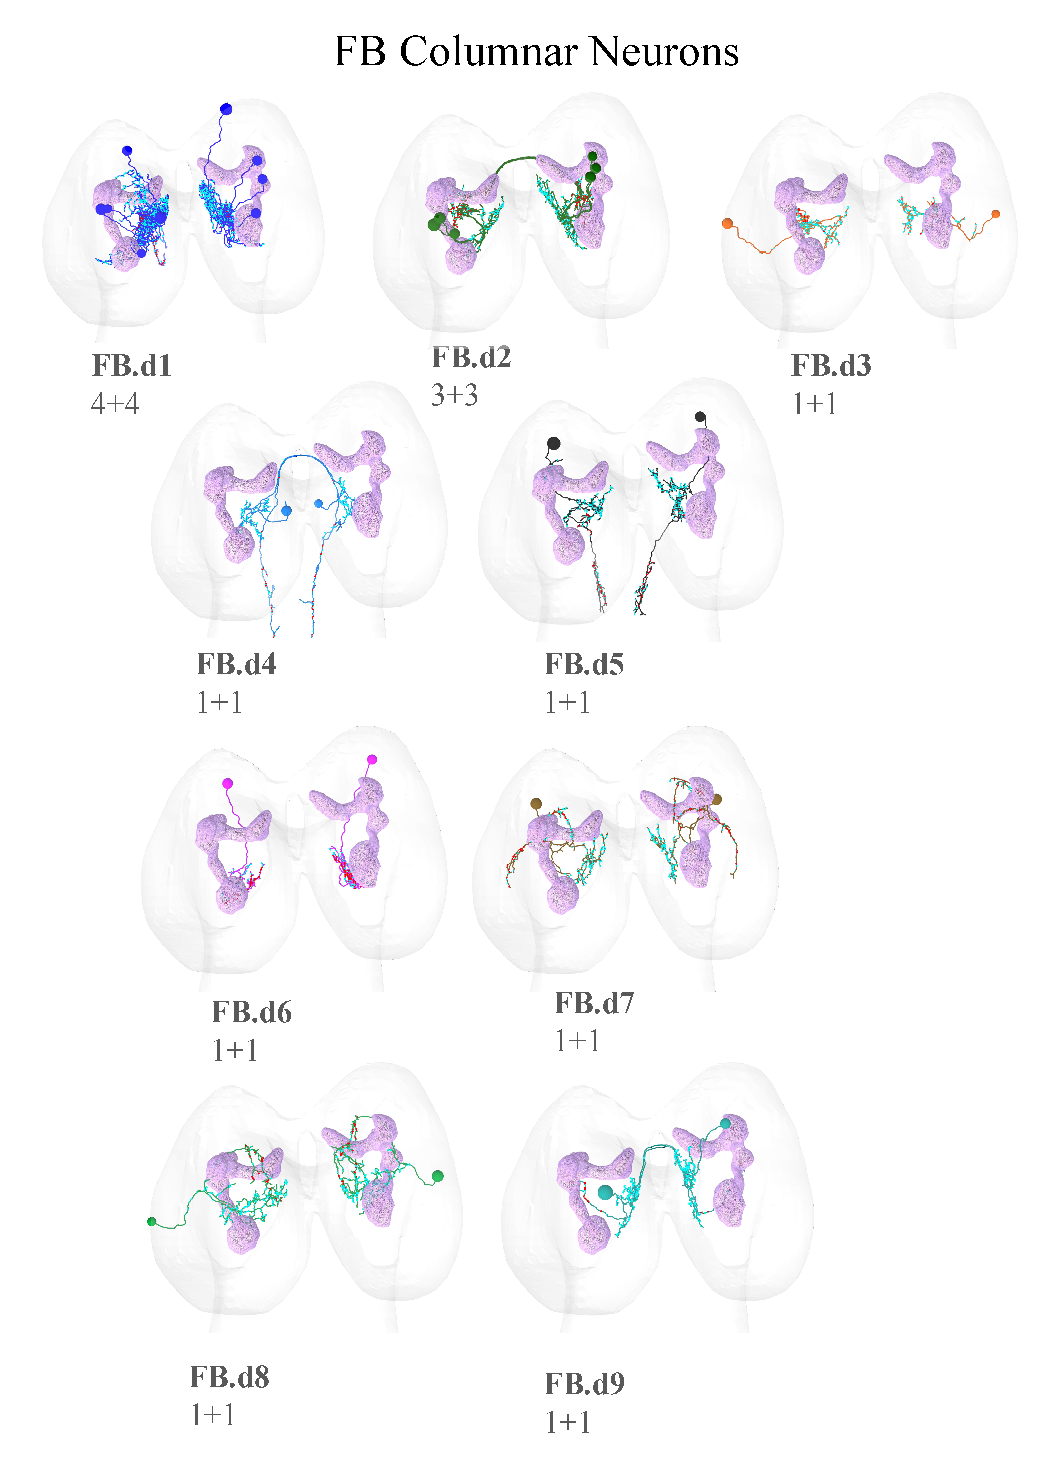
\includegraphics[width=15cm]{Figs/CX/FBColumnar.pdf}
        \caption[FB Columnar Neurons]{FB Columnar Neurons}
        \label{FBColumnar}
    \end{figure}


    In addition to generating FB tangential neurons, the DM1-DM4 lineages also contribute 5 pairs of FB columnar neurons. These neurons (FB.d.1) are characterized by ipsilateral-only dendrites largely circumscribed to the FB (except for the Bushy neuron from the DPMpm1/DM3 lineage), and projecting their ipsilateral-only clutchy axons solely the NO (so they are FB.d-NO.b). Therefore, FB.d.1 are specialized in relaying information from the FB to the NO hemilaterally. Among FB.d.1 we find CN-34, MB2ON-201 and MB2ON-204 \citep{eschbach2021circuits}. Importantly, 4 of the 5 FB.d1 pairs also send their dendrites to the PB, making them PB.d neurons as well, therefore PB.d-FB.d-NO.b as well as core cx neurons. This is the closest to the adult PFN, however the adult analogue would be PB.d-FBb.b-NO.b. %TODO refer figure with cx neurons analogues. 



    The DM lineage (larval CM4-vm lineage) further contributes 1 pair of neurons (FB.d.4) with ipsilateral dendrites in the posterior FB and beyond into an area adjacent to the LAL medially, and a contralateral axon that descends into the VNC, dropping presynaptic sites from the SEZ to the most posterior abdominal segments. Within the brain, FB.d.4 synapses onto some NO.d neurons (e.g., MB2ON-200) and also onto CN-28 \citep{eschbach2021circuits}.

    The MB neuroblasts contribute 3 pairs of early-born, non-Kenyon cell neurons (the 'ni' for "non-intrinsic"), named FB.d.2, with ipsilateral dendrites in the FB and a contralateral axon targeting exclusively the LAL.

    Then there are a collection of single pairs of neurons, each contributed by a different neuroblast, with dendrites in the FB and their axons targeting widely divergent neuropils, across the brain and also into the SEZ and VNC.

    The larval BLAv12 lineage contributes 1 pair of neurons (FB.d.3) with ipsilateral dendrites in the FB and also more medially, and ipsilateral axons targeting exclusively the LAL.

    The larval DALcm12-v lineage (adult CREa1) contributes 1 pair of neurons (FB.d.5) with ipsilateral dendrites in the FB and in the area adjacent but medial and ventral to the LAL, projecting their axons ipsilaterally from the NO to the medio-ventral brain and dorsal SEZ. The axons synapse onto a large number of NO.d neurons.

    The BAmv12-dor larval lineage contributes 1 pair of neurons (FB.d.6) with compact ipsilateral dendrites within the FB, and a compact short ipsilateral axon immediately dorsal on the PB. The FB.d.6 hence serve as a direct relay from the FB to the PB, synapsing onto half a dozen PB.d neuron types.

    The BAla12 larval lineage contributes 1 pair of neurons (FB.d.7; also known as FFN-6, \citep{eschbach2021circuits}) with compact ipsilateral dendrites in the FB, and an ipsilateral axon that targets the superior anterior protocerebrum where it synapses profusely onto the dendrites of DANs and OANs of the MB (DAN-i1, DAN-j1, DAN-c1, OAN-g1). Hence, FB.d.7 serves as a relay between the FB and the MB input neurons, conveying teaching signals for associative memories.

    The BLAl larval lineage contributes 1 pair of neurons (FB.d.8) with ipsilateral dendrites within the FB but also extensively lateral to the FB, and with peculiarly curving axons that follow the neuraxis, closely apposed to the dendrites of some hs-FB subtypes (hs-FB.1, hs-FB.2, hs-FB.3) and synapsing onto them.

    The DPMl2 larval lineage contributes 1 pair of neurons (FB.d.9, also known as FB-LAL1) with ipsilateral dendrites on the posterior  hemilateral FB (with inputs from hs-FB.2, hs-FB.5, hs-FB.6) and also reaching into the PB (with inputs only from ADC1), and a contralateral axon targeting the LAL where they synapse onto LAL LNs, EB.d neurons, and multiple descending neurons (DNs) that project to the SEZ and VNC.

    Finally, 3 of the 4 pairs of HF-PB neurons (the ones with a doubly crossing axon) are all FB.d, namely, they have dendrites within the FB and receive numerous synapses from FB.d neurons, in particular subtypes hs-FB.2, hs-FB.5 and hs-FB.6 (with further but weaker inputs from other subtypes). This indicates that the PB horizontal fibers not only integrate inputs from multiple sensory systems and gated by MB outputs, but are also modulated by the FB.

    % TODO the 4th pair of HF-PB neurons needs a distinctive name or tag.

    \begin{table}[ht]
    \centering
    \resizebox{\textwidth}{!}{%
    \begin{tabular}{l|ccccccccc}
    \toprule
    & \multicolumn{9}{c}{\textbf{FB Columnar}} \\
    \cmidrule(lr){2-10}
    \textbf{FB Tangential} & FB.d.1 & FB.d.2 & FB.d.3 & FB.d.4 & FB.d.5 & FB.d.6 & FB.d.7 & FB.d.8 & FB.d.9 \\
    \midrule
    hs-FB.1 & \cellcolor{forest5}70 & \cellcolor{forest3}10 & \cellcolor{forest2}6 & \cellcolor{forest3}16 & \cellcolor{forest4}25 &  & \cellcolor{forest4}54 & \cellcolor{forest2}2 &  \\
    hs-FB.2 & \cellcolor{forest5}145 & \cellcolor{forest4}68 & \cellcolor{forest3}24 &  & \cellcolor{forest4}43 & \cellcolor{forest2}8 & \cellcolor{forest2}2 & \cellcolor{forest3}19 & \cellcolor{forest4}30 \\
    hs-FB.3 & \cellcolor{forest4}35 & \cellcolor{forest3}19 &  &  &  & \cellcolor{forest3}19 & \cellcolor{forest3}18 &  & \cellcolor{forest2}1 \\
    hs-FB.4 & \cellcolor{forest2}3 & \cellcolor{forest2}4 &  &  &  &  & \cellcolor{forest3}21 & \cellcolor{forest2}1 &  \\
    hs-FB.5 & \cellcolor{forest3}18 & \cellcolor{forest2}2 & \cellcolor{forest1}1 &  &  &  & \cellcolor{forest2}1 & \cellcolor{forest2}1 &  \\
    hs-FB.6 & \cellcolor{forest5}166 & \cellcolor{forest4}41 & \cellcolor{forest3}11 &  & \cellcolor{forest3}6 &  & \cellcolor{forest2}1 & \cellcolor{forest3}19 & \cellcolor{forest3}18 \\
    hs-FB.7 & \cellcolor{forest4}63 & \cellcolor{forest3}16 & \cellcolor{forest3}10 &  &  & \cellcolor{forest2}8 & \cellcolor{forest4}50 & \cellcolor{forest2}1 & \cellcolor{forest3}19 \\
    hs-FB.8 & \cellcolor{forest3}8 & \cellcolor{forest2}4 &  &  &  &  & \cellcolor{forest2}5 & \cellcolor{forest2}1 & \cellcolor{forest2}1 \\
    \bottomrule
    \end{tabular}
    }
    \caption{Connectivity between FB Tangential and FB Columnar neurons. Cell shading corresponds to relative connection strength (darker = stronger).}
    \label{tab:fb-connectivity}
    \end{table}

    \textbf{\textit{Larval FB intrinsic neurons}}

    % Neurons that are both FB.b and FB.d
    We found two pairs of neurons (MB2ON-125 and eDAN-2) that are both FB.d and FB.b, corresponding to the third type of adult FB neurons: the intrinsic.

    MB2ON-125 integrate inputs across many neuron types, from PB.d columnar neurons to LH output neurons.
    As the MB2ON-125 name indicates (see \citep{eschbach2021circuits}), it receives direct synapses from MBONs (just MBON-c1, but a strong connection).
    Fairly large, its dendrites span approximately the entire spatial domain of the putative larval FB.
    Postsynaptically we find the CSD neuron \citep{berck2016wiring} and ascending neurons from the ventral nerve cord~(VNC), among many others such as FFN-31 (so-called feedforward neurons, from the MB perspective, that bring sensory inputs to MB DANs; \citep{eschbach2021circuits}).

    % DPMpl12
    eDAN-2 is a non-MB dopaminergic neuron (DAN) entirely circumscribed to the posterior-lateral end of the FB. See section on DANs of the CX below for details.


    \subsection{Noduli}
    \label{NO}

    In the larva we found a set of 21 neurons (10 pairs plus one unpaired) with highly compact, clutchy axons situated in the posterior ventral area of the brain, from lineages DPMm1 (DM1 in the adult), DALcm12, DPMl12, DPLc5, and BAMv12, as well as a few other larval lineages.
    We define the volume encapsulating all their clutchy axons as the putative Noduli of the larval \textit{Drosophila}, and labeled all these neurons as NO.b.

    Among the 21 NO.b neurons in the larva we find FB.d neurons (four pairs of the 5 FB.d.1 subtype including CN-34), convergence neurons (CN-6, CN-16/MBON-p1 \citep{eschbach2020recurrent}), neurons postsynaptic to MBONs (MB2ON-37, MB2ON-241), NO-looper (lineage BAmv12dor), MBON-p1 (a multi-compartment MBON of the MB vertical lobe; \citep{eichler2017complete}), and an unpaired neuron (DLPc lineage). Most NO.b neurons integrate inputs from the MB, as their names indicate (see \citep{eschbach2021circuits}).

    \begin{figure}
        \centering
        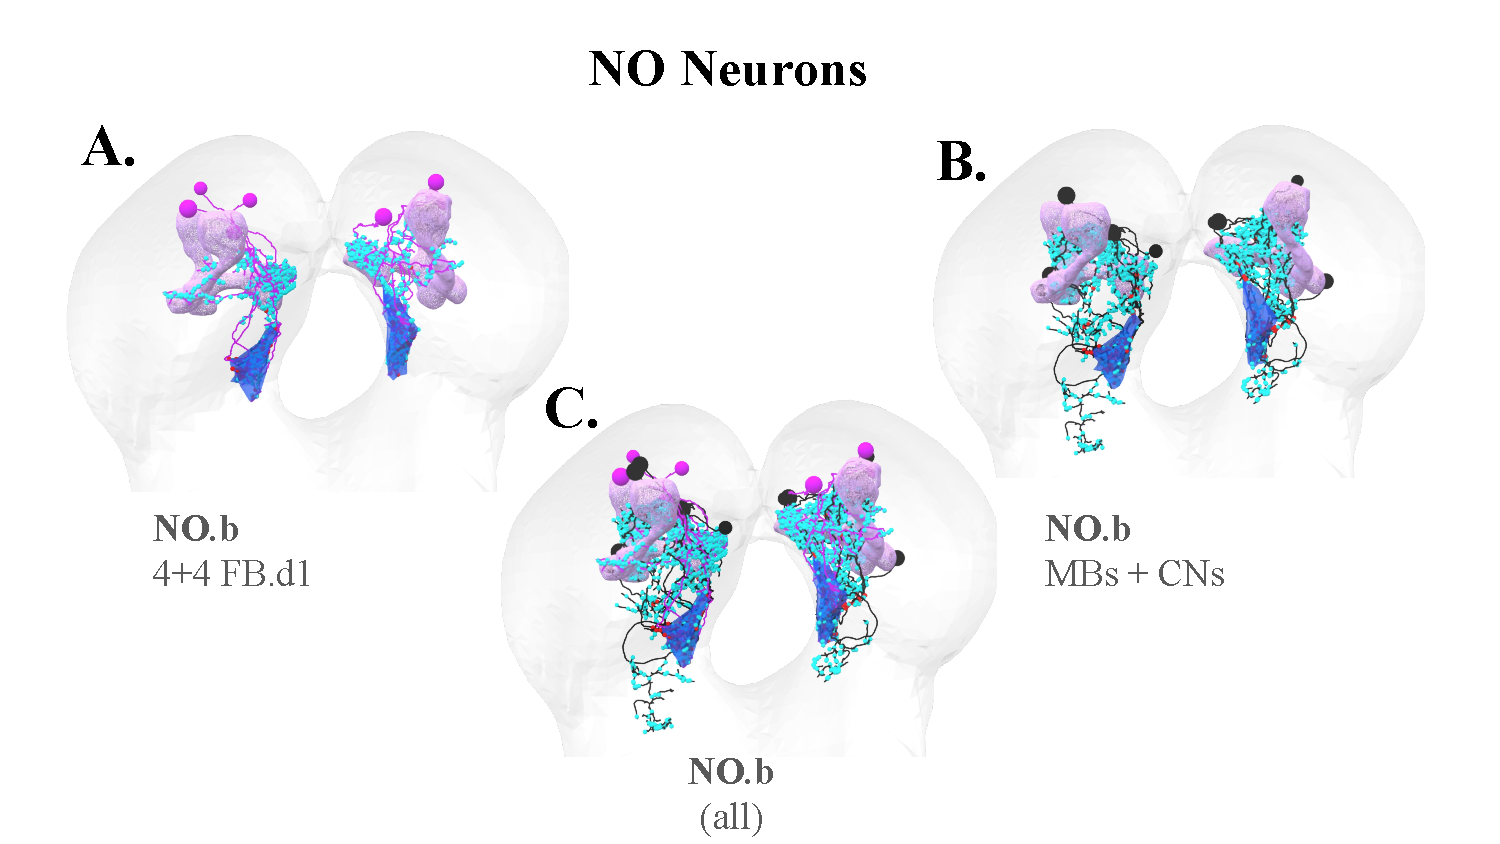
\includegraphics[width=14cm]{Figs/CX/NOneurons.pdf}
        \caption[Noduli Neurons]{...}
        \label{fig:label}
    \end{figure}

    Not a single NO.d neuron projects its axon onto any of the other core larval central complex neuropil, but some project to the LAL (Table \ref{inputsoutputs}), supporting a role for the NO as an output neuropil of the central complex.



    %In the putative larval NO, we find that the neurons projecting onto this neuropil receive input from LAL, (LAL.d MB2ON-75)

    %%17 MAY
    %Larval NO - 
    %recurrent connections exist but they are axo-axonic - 
    %most outputs are to MB2ONs, CNs, 10 pars of CNs, mostly MB related neurons. 
    %inputs are mostly multicompartment MBONs. 
    %TODO: no.d s should be the analogus to LNOs. 
    %TODO: find all LAL NEURONS, pk_lal is the volume. LALbs and LALds neuron search : annotation - larval central complex, check everything that is LAL something . look at those that have fullly encolsed synapses -  the lal columns have boh dendrites and axons fully contained in the volumes 
    %VMCc add it to the LAL. that is the LAL 


    %The NO receives inputs from LNO neuron types that innervate accessory structures: LAL, GA, and CRE. 
    % TODO check these set of synaptic connections
    %The majority of NO outputs (of CX columnar neurons) are to other CX columnar neurons (usually of the same type), or to LNO neurons that then provide input to the CX columnar neurons.
    %TODO: check if recurrence is axo axonic - 
    %todo: check if LNO1,2,3 check if they are actually the same as NO.b 
    %NO is synaptically interconnected with the other CX neuropils. All columnar neurons (PFNs and PENS) that synapse onto NO (are NO.b) are recurrently connected to the same LNO neurons they receive input from. 
    %PEN and PFN send output and recieve inputs from NO
    %LNOs mainly send outputs
    %Important comment against NO being an output structure: The only CX columnar neurons that lend some credence to the notion of the NO being an output structure of the CX are the PEN_b neurons, which provide strong inputs to the ExR8 neurons ()


    %%Sensory information
    %Many of these columnar neurons likely also receive input related to the fly’s self-motion in paired structures known as the noduli. 

    %In the adult Drosophila, the NO receives optic flow-based self-motion information and wind direction information via the columnar neurons.

    %an important hub for self-motion information according to physiological and anatomical observations. 
    % TODO In the larva, we find ... 16/21 receive inputs from MBONs, from PB (via 7 PB to noduli neurons, like in the adult), and from FB (some NO.b neurons are also FB.d neurons). 6/21 neurons are columanr neurons that aren't FB.d or PB.d or anything like that.

    %%Larva
    %In \textit{Drosophila} larva, we found a set of 21 neurons (10 pairs plus a confirmed unpaired neuron) with highly compact, clutchy axons clumped together in the posterior ventro-medial area of the brain (similarly to the adult NO) and belonging to neurons in lineages DM1 and DM3, as well as a few other larval lineages. We observe that these neurons are highly interconnected with the PB and FB,  with strong inputs from  PB and strong outputs to FB, and many of these neurons receive inputs in the LAL.
    %Their highly distinctive morphology, location as well as similarities in connectivity to the adult noduli, make these neurons an excellent candidate for the putative larval noduli.


    %TO DO: can we see the kind of specific recurrent activity

    % CONSIDER introducing the LAL but in the adult it is not considered a CX neuropil
    % \subsection{The new LAL}

   


\section{Mushroom Body and the Central Complex}
    In the adult \textbf{Drosophila}, the Mushroom Body is known to output onto the Central Complex neuropils through the MB Output Neurons (MBONs). At this stage, adult MBONs primarily target the Fan-shaped Body - tangential neurons from the middle layers (4-6) - and the Noduli - via a direct glutamatergic connection from MBON-30 to LCNOp(LAL–NO) neurons which then target the PFN (PB-FB-NO) neurons \citep{hulse2021connectome}.Here, we examine the synaptic relationships between mushroom body input (DANs, MBINs, OANs) and output (MBONs) neurons and the larval central complex neuropils. 
        
    \begin{figure}
        \centering
        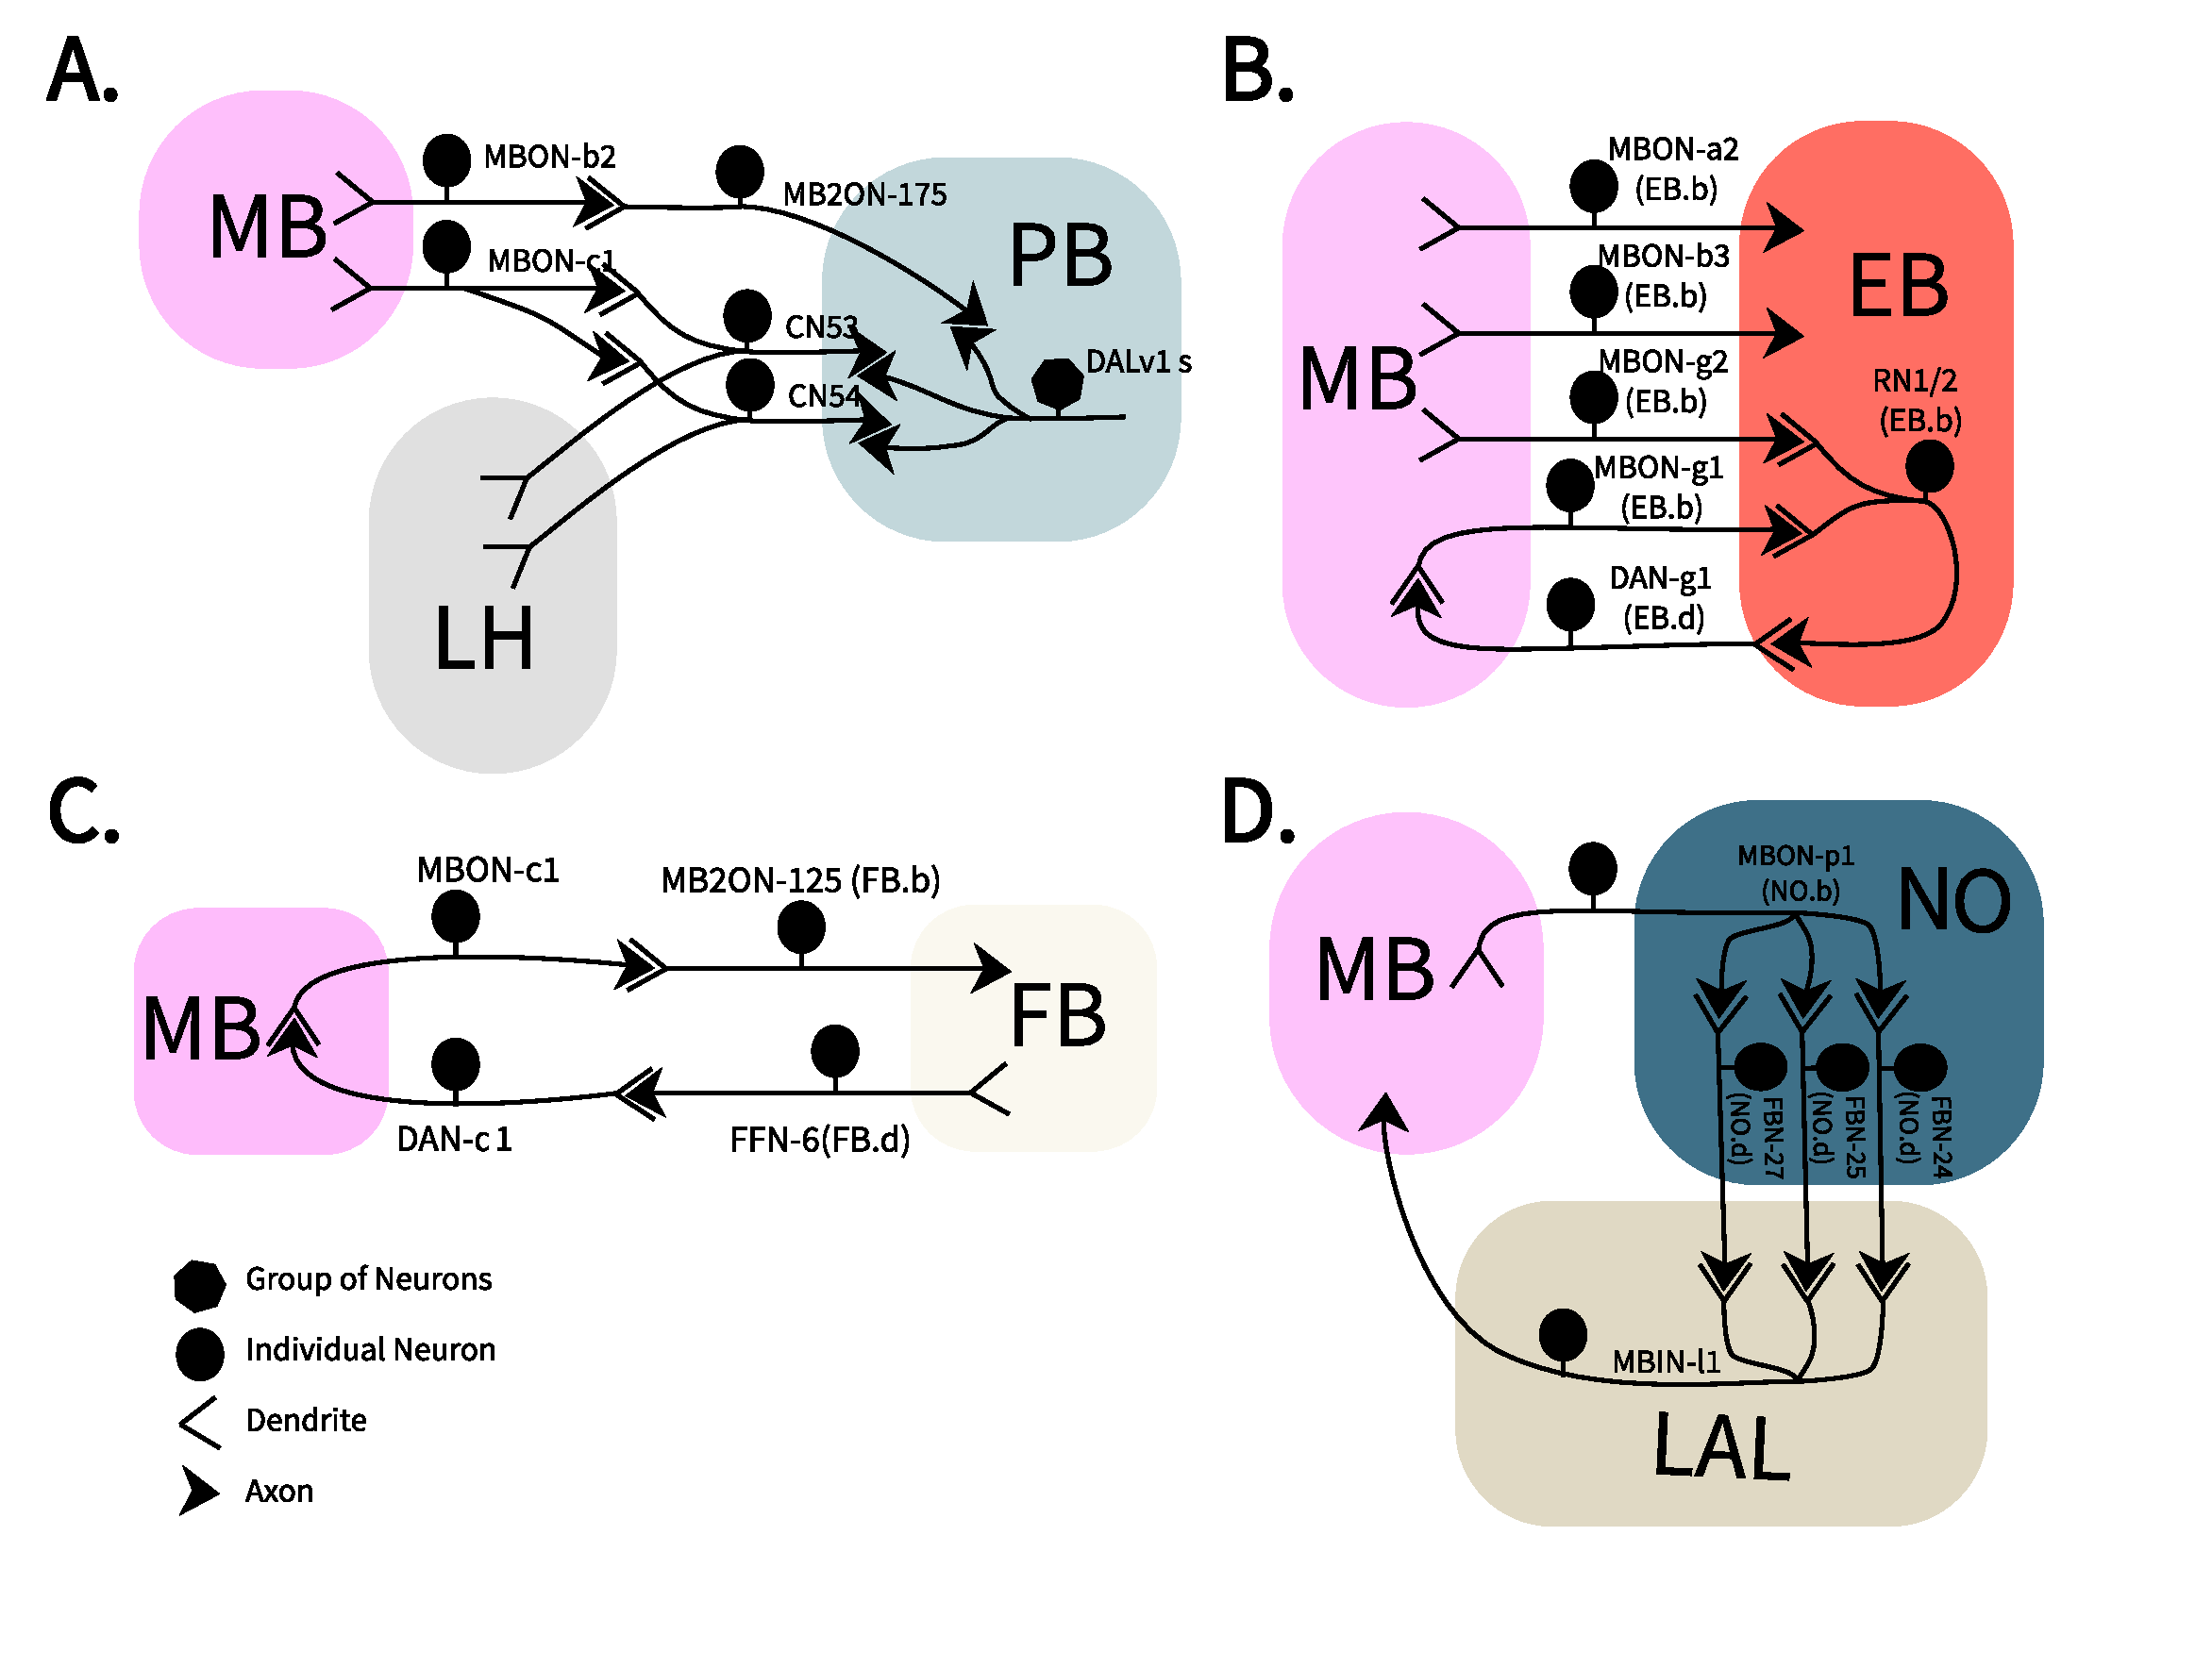
\includegraphics[width=17cm]{Figs/CX/MBtoCX.pdf}
        \caption[Mushroom Body Connections to the Larval CX]{Mushroom Body Connections to the Larval CX}
        \label{MBtoCX}
    \end{figure}

    \subsubsection{A loop between FB and the 'c' compartment of the MB}
    % MBON-c1 -> MB2ON-125 (FB.b) -> FFN-6 (FB.d) -> DAN-c1  
    We found that MBON-c1 synapses onto one FB.b neuron, MB2ON-125.
    Interestingly, DAN-c1 integrates inputs from an FB.d neuron, FFN-6, which in turn integrates inputs from a few neurons that are directly postsynaptic to MB2ON-125, defining a loop between the MB 'c' compartment and the FB.
    No other MBON supplies direct or two-hop inputs onto the FB.

    % EB to MB
    \subsubsection{Reciprocal connectivity between EB ring neurons and the 'g' compartment of the MB}
    % axo-axonic then axo-dendritic:
    % MBON-g1/g2 (EB.b) -> RN1/2 FBN-20 -> DAN-g1 (EB.d)
    Four MBONs (a2, b3, g1 and g2) are EB.b (i.e., deliver synapses to the EB; Fig. \ref{fig:mbtocx}). Interestingly, some of these MBONs are monosynaptically interrelated, namely MBON-g1 and -g2 (which promote approach) are GABAergic neurons that synapse onto MBON-a2 (which promote avoidance) \citep{eschbach2021circuits}.
    Furthermore, MBON-g1 and -g2 synapse axo-axonically onto an EB ring neuron, RN1/2 (also known as FBN-20; \citep{eschbach2021circuits}), a core GABAergic neuron of the EB, which in addition to synapting axo-axonically recyprocally onto EB wedge neurons also synapses onto an EB.d neuron, DAN-g1.
    Therefore, the output of the MB 'g' compartment (MBON-g1 and -g2) modulate, with GABA, the axon of an EB ring neuron (RN1/2), which in turn synapses onto the dendrites of the teaching neuron of the MB 'g' compartment (DAN-g1).
    This circuit configuration defines a close relationship between an associative learning compartment (MB 'g') and the EB.

    Assuming the larval ring neurons RN1/2 are also GABAergic, as they are in the adult \citep{hanesch1989neuronal}, the MB 'g' compartment is providing disinhibitory input onto the EB, by means of MBON-g1/g2 inhibiting its ring neurons.
    This disinhibition could be understood as a learning-based gating mechanism over EB wedge neurons, with features of input space expressed in the Kenyon cell population code, by coincident activity with DAN-g1, modulating the activity of the EB wedge neurons that the ring neurons also synapse onto.
    Taken together, this implies that, if the larval EB is functionally similar to that of the adult EB, there is a component of learning built-in into the internal representation of the direction of movement.

    \subsubsection{A loop between the NO and the MB vertical lobe via the LAL}
    % All are axo-dendritic synapses:
    % MBON-p1 (NO.b) -> FBN-24/25/27 (NO.d) -> MBIN-l1

    MBON-p1 is a multi-compartment MBON of the MB vertical lobe that is an NO.b, (i.e., it delivers output synapses to the NO).
    At the NO, MBON-p1 synapses onto several NO.d neurons, FBN-24, FBN-25, and FBN-27, which are MB feedback neurons \citep{eschbach2020recurrent} that all project to the LAL and synapse strongly onto MBIN-l1, a MB input neuron targeting multiple compartments of the vertical lobe.
    This circuit configuration defines a strong tight loop between the MB vertical lobe and the NO via the LAL.

    Note that the dendrites of MBIN-l1 are entirely contained within the LAL compartment.
    In addition, these three feedback neurons also synapse weakly onto DAN-d1.


    \subsubsection{The MB modulates inputs to the PB}
    % MBON-d1 -> MB2ON-63 (PB.b) -> multiple PB.d (some are NO.b like MB2ON-241)
    % CN-53, CN-54, MB2ON-175 all synapse onto DALv1 neurons

    % VISUAL input to the PB and the EB
    Multiple sensory modalities converge onto the horizontal fibers of the PB (DALv1 neurons) via MB convergence neurons (CN-53, CN-54) and a neuron postsynaptic to MBONs (MB2ON-175).
    These CNs were previously described as integrating the output of both the lateral horn (LH), which conveys innate pathways, and the mushroom body (MB), for associative memory \citep{eschbach2021circuits}.
    Synapses from CN-53, CN-54 and MB2ON-175 onto PB horizontal fiber neurons (DALv1) follow an intriguing pattern of synapting onto either the dendrite or the axon, but largely not both, with specific target choices among the 4 DALv1 neurons.
    In considering that 3 of the 4 DALv1 neurons (PB horizontal fibers) present an unusual bilateral axon that first deploys output synapses contralaterally and then ipsilaterally (Fig. \ref{fig:dalv1neurons}A), the observed pattern of selective axo-dendritic and axo-axonic connections has implications for the modulation of the output of the unusual axons of DALv1 neurons.


    In summary, from the perspective of the PB, we find the following circuit architecture: the multi-sensory convergence onto the PB horizontal fibers is directly modulated by the MB, precisely because the neurons that mediate the multi-sensory convergence are themselves CNs (i.e., integrate also MBON synapses in addition to LH inputs): the CN-53 and CN-54. %Both of these neurons are also Lateral Horn (LH) neurons.
    Note CN-54 is in addition a PB.d neuron, integrating inputs from PB horizontal fibers (DALv1 neurons).

    Upstream, among various MBONs, MBON-c1 is the most strongly connected to both CN-53 and CN-54, which also integrate inputs from MBON-b1 and MBON-b2. All three are MBONs of the MB peduncle; MBON-c1 has no known function, while MBON-b1 and MBON-b2 promote approach \citep{eschbach2021circuits}.

    Of note, the axon of MBON-c1 receives direct presumably inhibitory (GABAergic) inputs from MBON-g1, MBON-g2, and MBON-d1, with all three MBONs participating of circuit loops with other central complex neuropils.

    Additionally, neurons directly postsynaptic to MBONs, such as MB2ON-175, in turn directly synapse onto the horizontal fibers of the PB, either axo-axonically or axo-dendritically, in a pattern selective of specific DALv1 neurons.

    In summary, not only are navigational decisions such as whether to turn to stimuli or not proceeding not independently per sensory modality but integrated across modalities, as observed before in behavioral experiments \citep{gepner2015computations}, but also such integration is modulated by prior memories.

    %Vertical lobe is used by the NO and MB and LAL.
    %mb2on-c1 has no results(when it comes to aversion), but massively related to EB so it might 
    %mb2in-l1 according to eschback all the compartments of vertical love are for aversive behaviour.only mnbin that is not bilateral.  
    %m2on-p1 noduli itself gets input from(..) 
    % (extended data figure 6a - complete connectome of learning memory centre) 
    % ipsilateral control via these only mbons and mbins that are ipsilateral as opposed to bilateral. 


















\section{Dopaminergic neurons (DANs) of the larval central complex}
    
    \begin{figure}
        \centering
        \includegraphics[width=17cm]{Figs/CX/DANs.pdf}
        \caption{Confocal Images of Immunostained Dopaminergic neurons of the Larval Central Complex}
        \label{DANs}
    \end{figure}

Dopaminergic release outside the MB in the adult fly is known to trigger sleep via dorsal FB (dFB) neurons~\citep{pimentel2016sleep}, among other potential roles, depending upon the dopamine receptors expressed in the postsynaptic neurons and the circuits the neurons are part of.

The larval MB houses 7 pairs of DANs \citep{eichler2017complete}, with several more DANs scattered across the brain \citep{selcho2009thgal4}. By flp-out of the TH-GAL4 expression pattern that encompasses all DANs \citep{selcho2009thgal4} followed by immunohistochemistry, we isolated individual neurons from the TH-GAL4 expression patteern and compared their morphology with EM-reconstructed brain neurons \citep{winding2023connectome}. We identified with reasonable certainty the following 5 eDAN types (eDAN for \textit{external} DAN, i.e., not a MB DAN), comprising 6 neuron pairs.

\textbf{eDAN-1}: from the larval lineage DPMpm2, this neuron presents an ipsilateral dendrite in the posterior-dorsal brain, and a bilateral axon exactly overlapping with HF-PB dendrites. eDAN-1 integrates inputs from PB.d neurons like CN-54 (which mediates multi-sensory input integration and relays them to HF-PB, modulated by MB output; see above) but also from multiple sensory PNs such as for temperature (Suckerfish PN, Thermo PN 3 and Thermo PN 5), olfaction (mPN A3), and for unknown sensory modalities (Suckerfish PN 2, from unknown sensory MN-Sens-B2-ACp-21 and -22; \citep{miroschnikow2018convergence}), and also from PB.b neurons like MB2ON-63. The axon of eDAN-1 synapses onto multiple PB.d neurons (MB2ON-187, CN-15, CN-54, ADC1, FB-LAL1, and SP2-1) and weakly onto HF-PB neurons.

\textbf{eDAN-2}: from the larval lineage CM4-dm, this DAN presents a small, compact ipsilateral dendrite and a contralateral axon on the corresponding contralateral hemisphere right at the posterior end of the FB. eDAN-2 integrates inputs from FB neurons (strongly from FB.d.6, hs-FB.3, hs-FB.1, and weakly from many more). Its axon synapses onto MB2IN-195 (which is presynaptic to EB Wedge neurons), multiple FB neurons (hs-FB.3, hs-FB.1, FB.d.7 (FFN-6)), and weakly onto MB2IN-191 (the octopaminergic VUM of the CX).

\textbf{eDAN-3}: also known as MB2IN-139 \citep{eschbach2021circuits}, this neuron is from the larval lineage DPMpl12. Its dendrite is ipsilateral, sitting lateral to the FB but also extending into the LAL. The eDAN-3 axon targets a region dorsal to the LAL, housing the dendrites of  many EB.d neurons onto which it synapses, such as MB2IN-114, EB-DN1, MB2ON-17, EB wedge neurons (only W1), and many more neurons such as convergence neurons (CN-30, CN-37, CN-38, CN-41, CN-42, CN-43), MB2ON-256, and a peculiar FB.d.1 neuron (Bushy).

\textbf{eDAN-4}: this type consists of two nearly identical neurons that share most inputs but differ only slightly in their outputs, since their axons are juxtaposed but tiled medio-laterally. From the larval lineage DPMpl12, they present an ipsilateral dendrite in the posterior ventral brain and a contralateral axon in the posterior intermediate brain, beyond the limits of the FB proper. Both integrate inputs from numerous EB.d neurons like MB2IN-124, but only eDAN-4l (lateral axon) receives synapse from hs-FB.3. The axons of both eDAN-4 synapse onto some NO.d neurons like MB2ON-248 (whose dendrite has a domain in the NO and another outside where it meets the axon of both eDAN-4) and of other unidentified neurons (lasso-top 3, DALcm12-v descending), but only eDAN-4l synapses onto convergence neurons (CN-9, CN-26), and only eDAN-4m synapses onto hs-FB.5 and hs-FB.7.

\textbf{eDAN-5}: from the DPMpm1 larval lineage, this neuron's dendrite lays posterior to the LAL and projects its axon inside the lateral LAL. The dendrite integrates inputs from EB.d neurons, MB2IN-195, MB2ON-67, and sVUM2mx. The axon targets weakly but axo-dendritically an EB Ring neuron (RN1/2), and more strongly other neurons (MB2ON-67, MB2ON-78, MB2ON-68).

According to \citep{selcho2009thgal4} there are further non-MB DANs yet to be identified in the larval brain connectome. Note an effort was made to relate the eDANs we could identify to non-MB DAN names in \citep{selcho2009thgal4} but the resolution mismatch was too great to bridge, except for eDAN-1 which is most likely named "DM3" in \citep{selcho2009thgal4}.

%TODO: add eDAN-6 and eDAN-7
%TODO: add connectivity between all DANs

\section{Behavioral Assays - Loss of Function Analysis during light stimulation}
    \begin{figure}
        \centering
        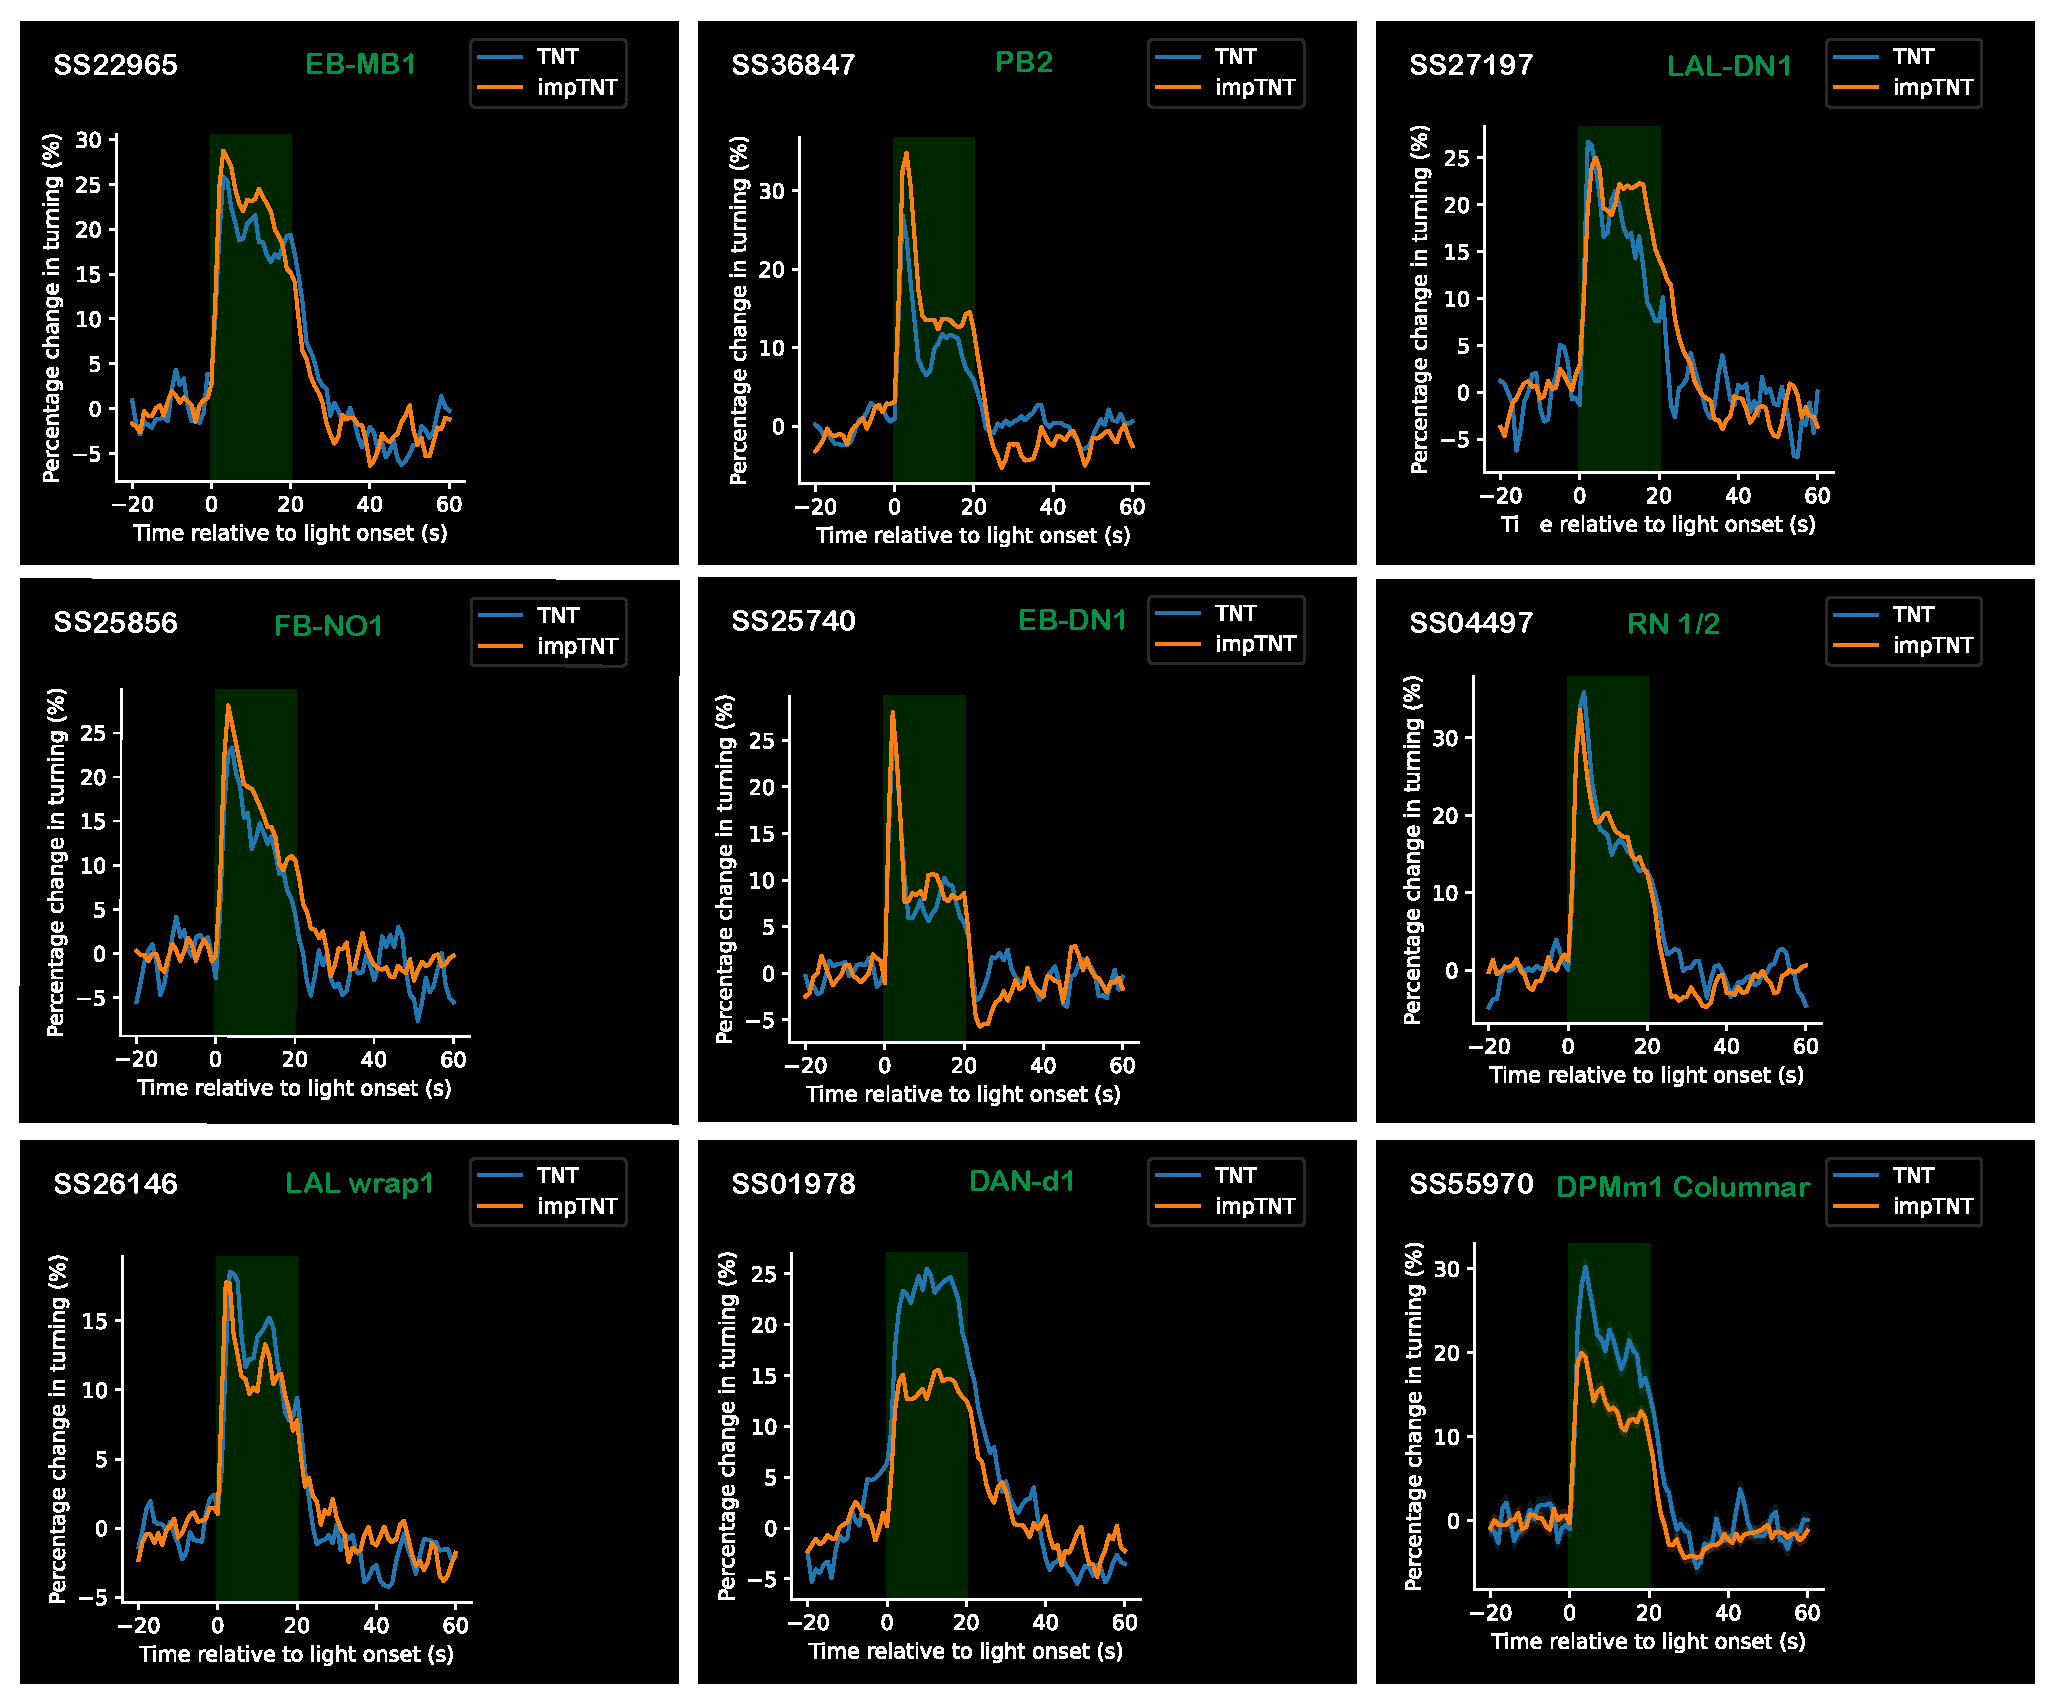
\includegraphics[width=12cm]{Figs/CX/BehaviourAssays.pdf}
        \caption[Loss of Function Analysis during Light Stimulation]{\textbf{Loss-of-function Behavioral analysis of CX neurons expressing TNT and impTNT(disabled TNT)} The name of each split GAL4 line is written in white and their corresponding neuron name in green. Stimulation via green light is highlighted in green from 0-20s. The plots show a time-series of larvae's turning rates, colored in blue for larvae expressing TNT and orange for larve expressing impTNT}
        \label{LOS}
    \end{figure}

    We identified genetic driver lines for eight neurons of the larval central complex: EB-MB1, PB2, LAL-DN1, LAL wrap1, FB-NO1, EB-DN1, RN1/2, plus DAN-d1, which is an EB.d (i.e., integrates inputs from the EB). 
    We quantified larval turning behavior following targeted inhibition of each of these driver lines via Tetanus neurotoxin (TNT).
    Control animals expressed the inactive variant, Impotent Tetanus (ImpTNT).
    Given that the central complex is classically implicated in visually guided navigation, we used green light stimulation as the sensory stimuli.
     \begin{table}[h!]
    \centering
    \begin{tabular}{llllll}
    \toprule
    \textbf{Neuron Name} & \textbf{Other names} & \textbf{Split Line} & \textbf{.b} & \textbf{.d} & \textbf{Lineage} \\ 
    \midrule
    DAN-d1      &   FB-33         & SS01978 &       & EB.d        & CPb        \\ 
    LAL wrap 1  & MB20N-116       & SS26146 &       & LAL.d       &  DALcl12-v  \\ 
    FB-NO 1     &                 & SS25856 & NO.b  & FB.d        &  DPMl12    \\ 
    EB-MB 1     & FB2IN-12(Mickey Mouse)& SS22965 &       & EB.d    & BLP1/2    \\ 
    RN 1/2      & FBN-20, MB2IN-38 & SS04497 & EB.b  &             &  DALv23    \\ 
    EB-DN 1     & MB20N-75        & SS25740 &       & EB.d, LAL.d & DPMpm1 \\ 
    LAL-DN 1    &                 & SS27197 &       & EB.d            & DALd   \\ 
    PB2         & PB horizontal fibers & SS36847 & PB.b      &             & Dalv1  \\ 
    \bottomrule
    \end{tabular}
    \caption{ \textbf{Neurons tested for LOF} Neuron names, corresponding split GAL4 line used for LOF experiments, and lineage information.}
    \end{table}

    We found that expressing TNT did not show significant changes to turning rates for most neurons when compared to controls in response to green light stimulation, with the exception of DAN-d1 \ref{LOS}. 

    % TODO consider creating above a separate subsubsection for DAN-d1
    % To investigate their contribution to navigation and to test the hypothesis that they function as components of a navigational center, – DISCUSSION


\section{Neural activity in response to blue light stimulation}
We were curious if the identified putative central comlpex would be responsive to light stimulation. 
We monitored the activity across the entire larval brain in response to stimulation of Rh5 (blue senstitive) phtoreceptors. Photoreceptors (the Bolwig Organ) are located outside of the Central Nervous System(CNS) of Drosophila. We thus expressed  EGFP fluorescent tag in these neurons(Rh5s) to be to ensure they are present during dissection of the CNS and that they are preserved for mounting the sample in the glass capilary prior to Calcium Imaging. We created a final line that expresses green fluorescent RGECO (a calcium indicator of neural activity present cytosl) and red fluorescent IRFP (which brightens the cell nuclei very well and allows visualisation of cell position) and green fluorescent Rh5 photoreceptors. 


Upon blue light stimulation, robust calcium transients in multiple regions of the larval brain were observed. Amongst the CX neuropils, we expected the neuropil with the most visual input (Protocerebral Bridge) to be realiably responsive to photoreceptors. To test this, the brain was segmented into distinct anatomical regions using manual annotation. Regions corresponding to the optic lobe (OL) - to confirm functional photoreceptors - the putative Protocerebral Bridge, and the MB - as a control -  were delinated (Fig. \ref{LSSegmentation}).
based on anatomical landmarks and lineage tracing data. Flu orescence intensity changes $\Delta F/F_0$ were quantified for each region before, during and after blue light stimulation. 

   \begin{figure}
        \centering
        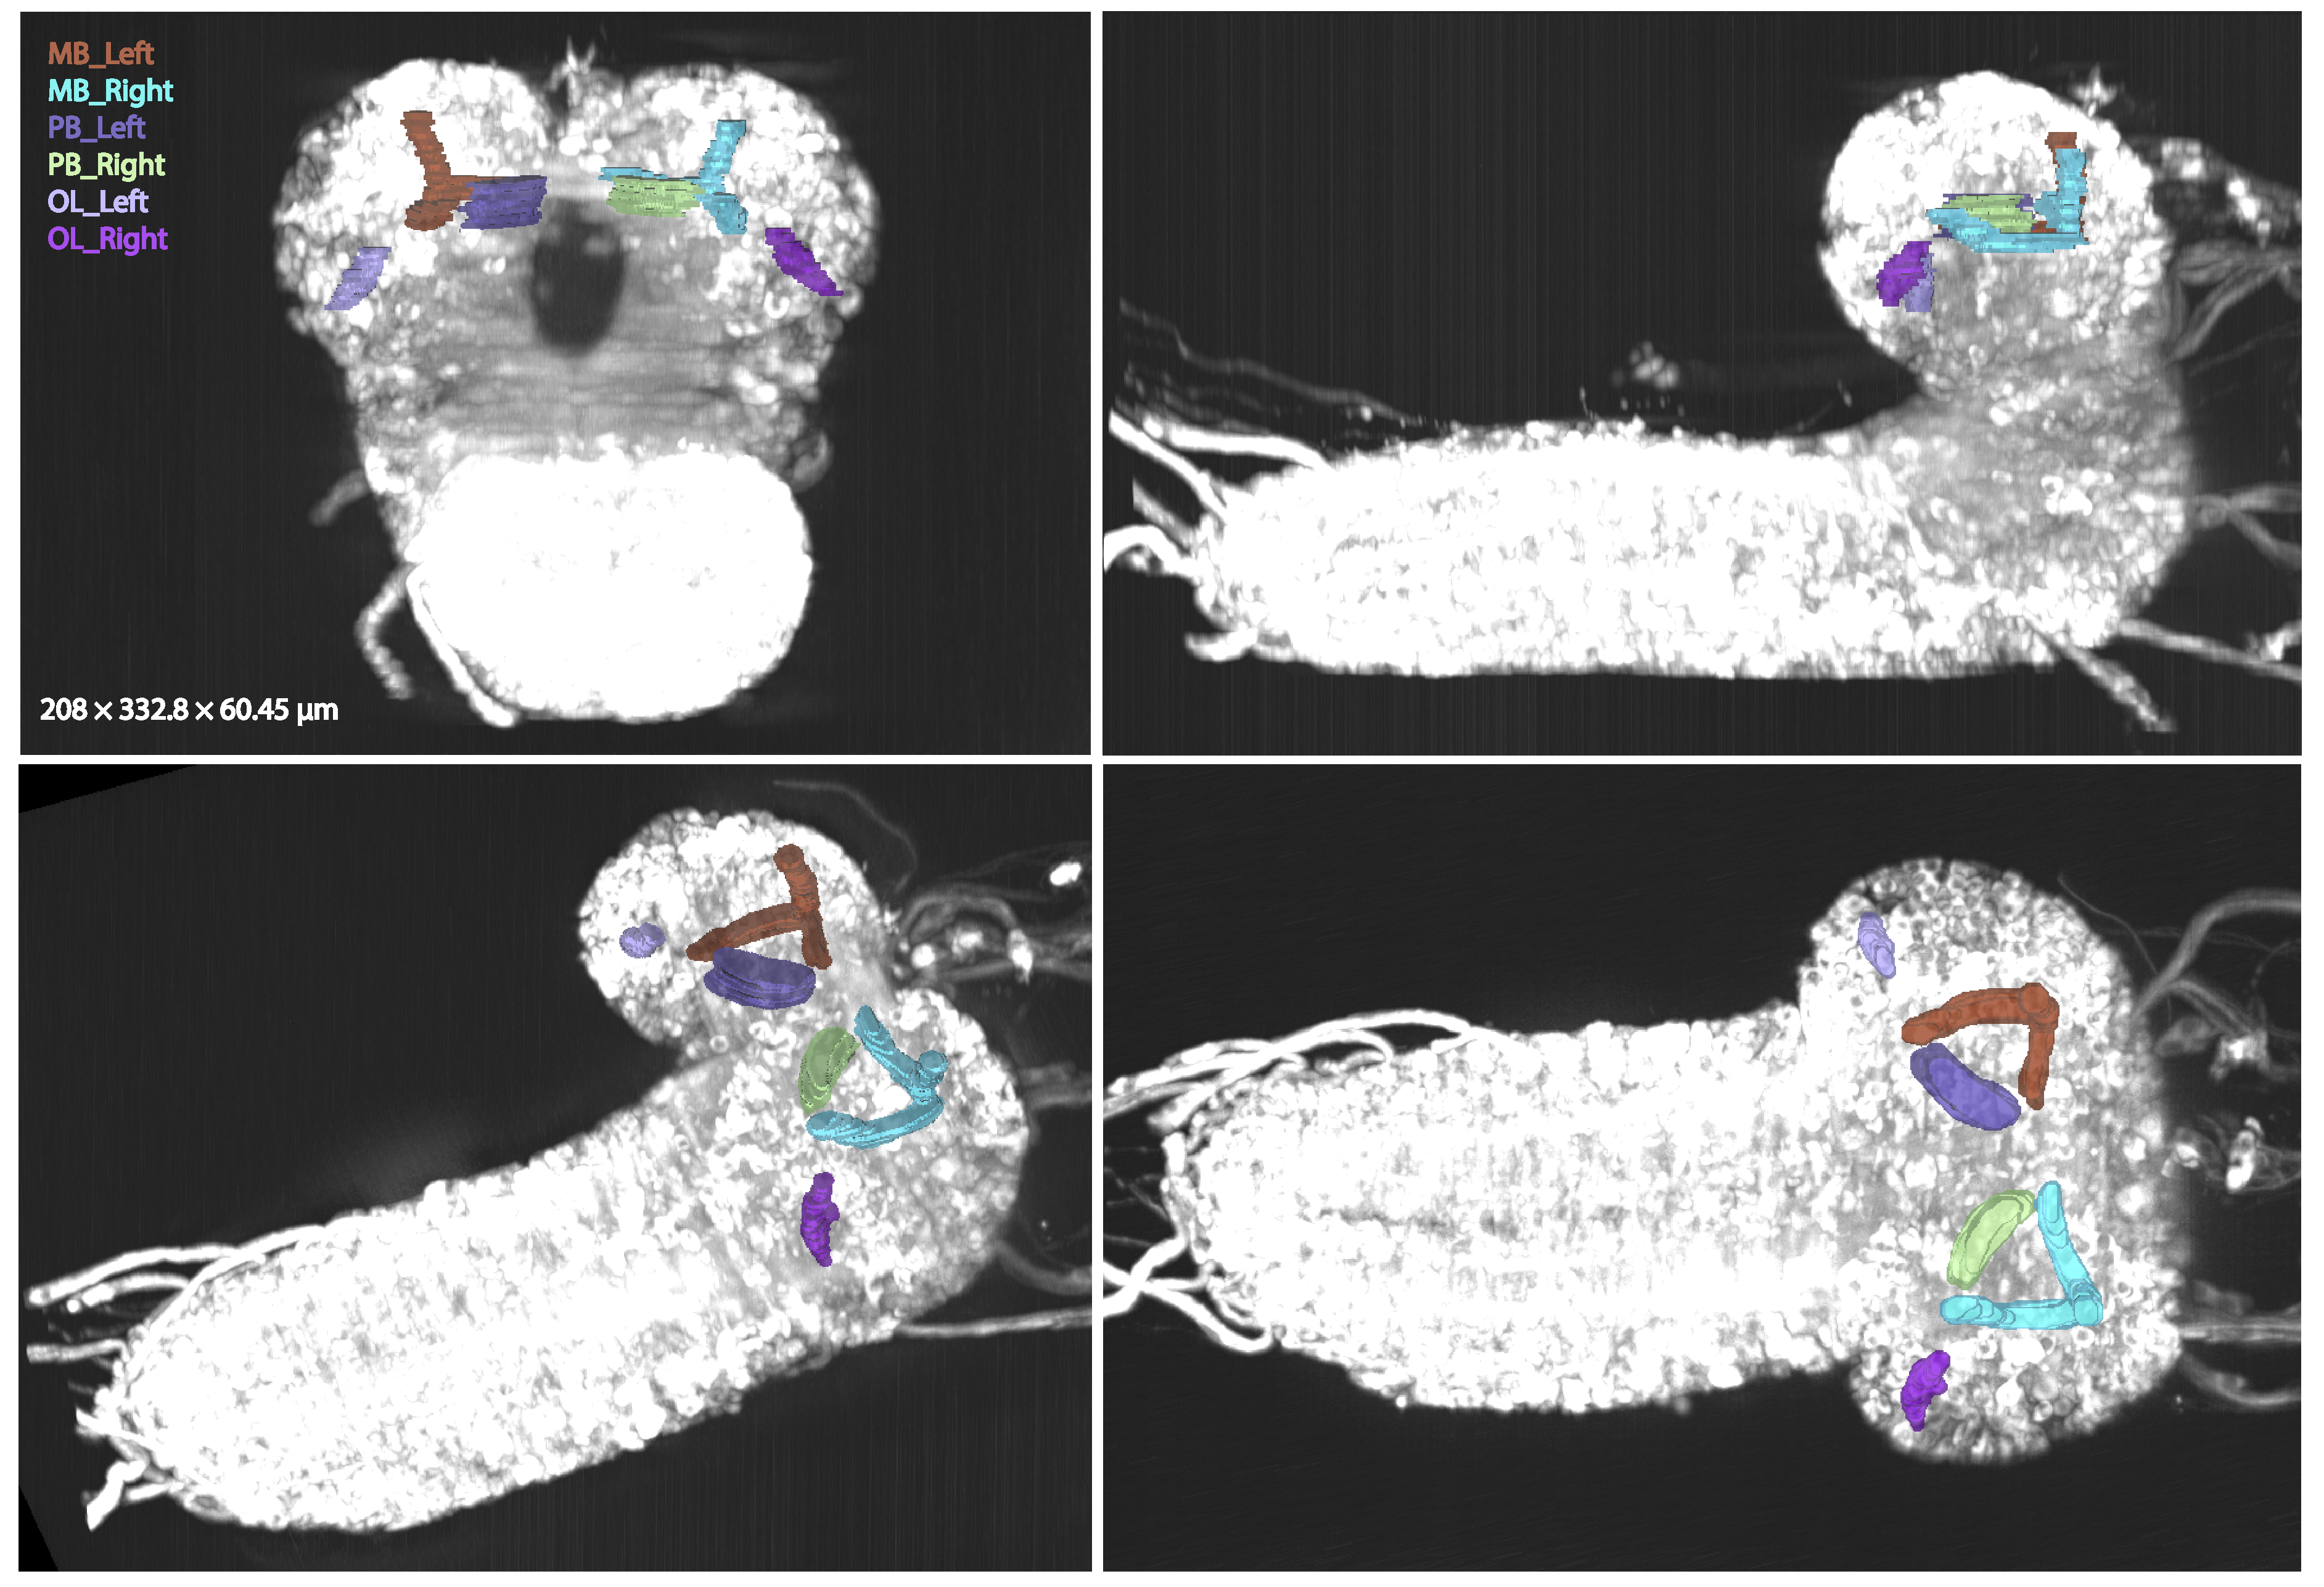
\includegraphics[width=10cm]{Figs/CX/LSSegmentation.pdf}
        \caption[Lightsheet volume Segmentation]{Lightsheet Volume Segmentation}
        \label{LSSegmentation}
    \end{figure}

The Optic Lobe (OL) was reliably activated in response to light in sample 1,3 and 5 samples which confirms intact and functional photoreceptors. For sample 2 the left OL significanlty less responsive than the right, indicating possible tissue damage on that side of the brain. Similarly for sample 4 the right side is less responsive than the left. 
Notably, across all samples, the OL exhibited a markedly larger $\Delta F/F_0$ response compared to other regions of interest, creating a masking effect in data visualization. Specifically, the large amplitude of OL activity expanded the y-axis range, compressing the apparent variability in other regions and obscuring meaningful differences between the PB and the MB. To better resolve the relative dynamics among the remaining regions, the OL traces were excluded from subsequent analysis and the data was replotted and presented side by side with the original in figure \ref{LSanalysis}. 

 
    \begin{figure}
        \centering
        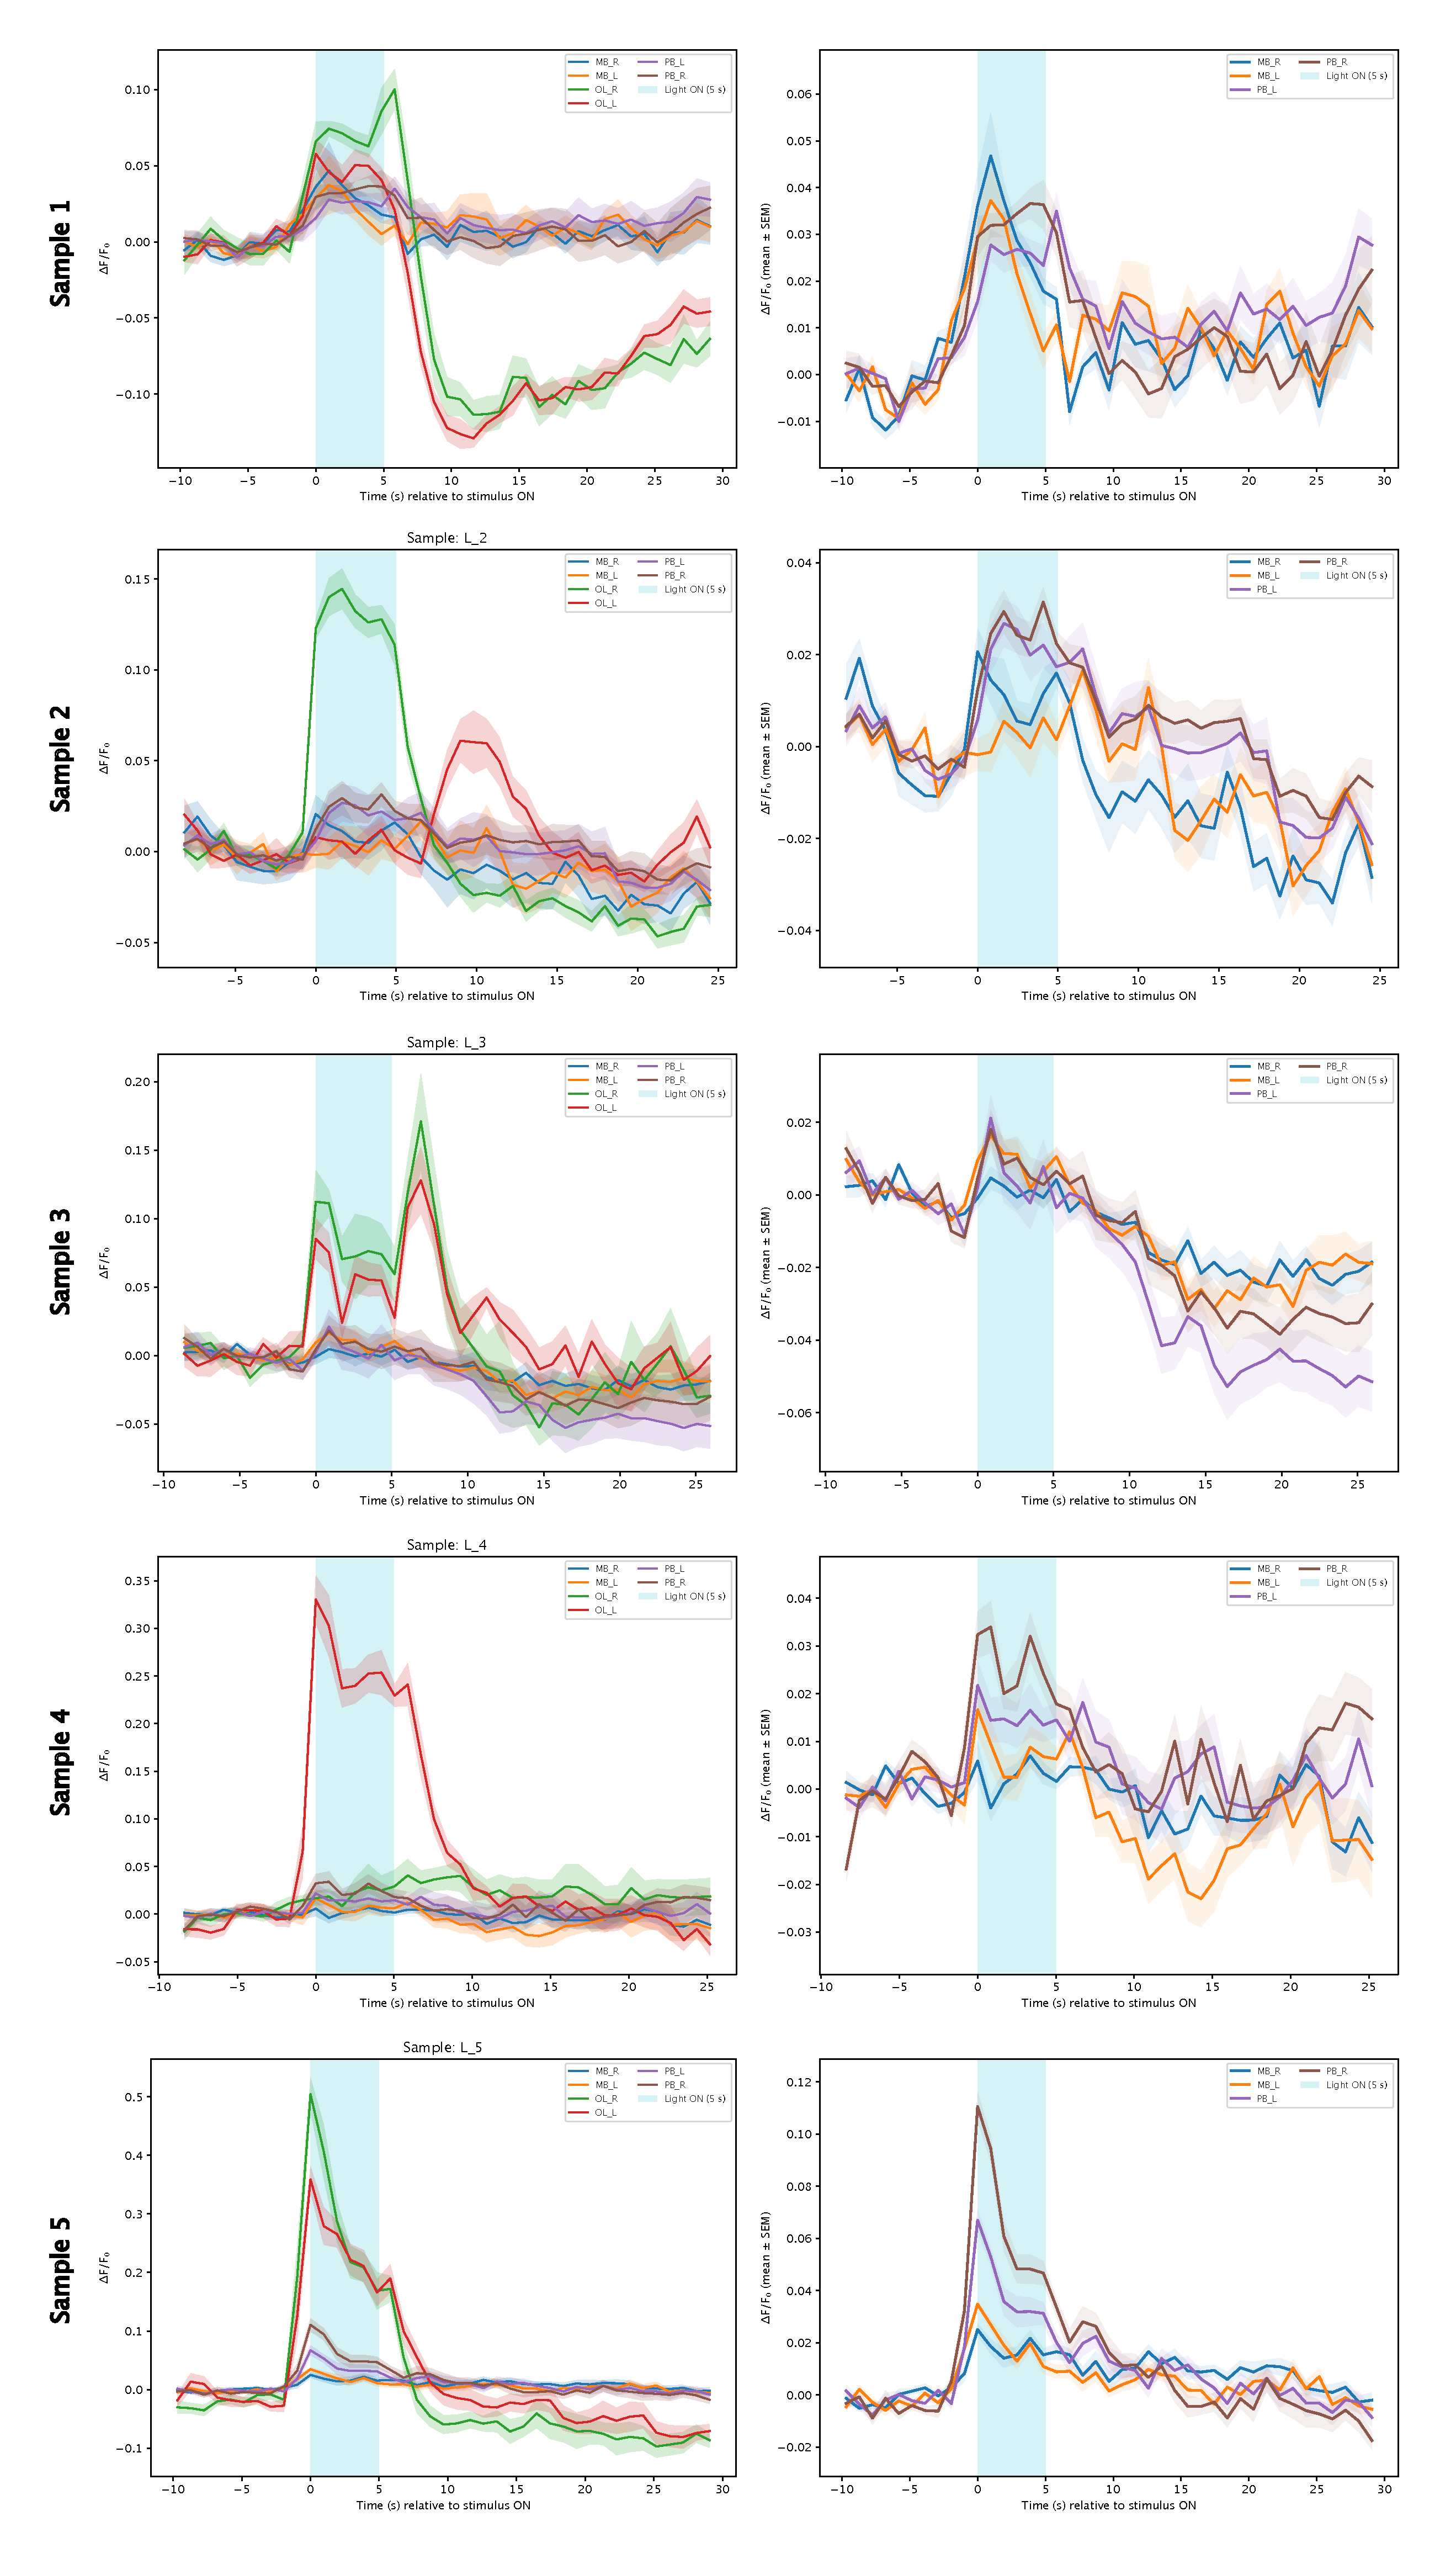
\includegraphics[width=10cm]{Figs/CX/LSanalysis.pdf}
        \caption[Neural Activity of the Larval Brain in response to Photoreceptors Rh5 Stimulation]{Neural Activity of the Larval Brain in response to Photoreceptors Rh5 Stimulation}
        \label{LSanalysis}
    \end{figure}


When compared to the control (MB), the larval Protocerebral Bridge (PB) exhibited higher amplitude calcium transients in samples 2, 4, and 5, whereas both neuropils showed similar activity in samples 1 and 3. Interestingly, the two samples with one inactive optic lobe (samples 2 and 4) displayed a more pronounced difference between PB and MB activity, suggesting that unilateral OL impairment may enhance the relative responsiveness of the PB to visual stimulation. This observation may indicate compensatory mechanisms or altered circuit dynamics in the presence of partial sensory deprivation. 
Overall, there seems to be a higher sensitivity to blue light from in PB compared to the MB, supposrting the hypothesis of a functional role in visual input processing (Fig. \ref{LSanalysis}. However, the effects aren't as significant as expected, possibly due to small sample size, suggesting the experiment could be underpowered.


\section{Descending Neurons from CX}    
%catmaid annotation: 
                129 neurons descending to VNC
                93 neurons descending to SEZ
                216 total descending
                layer 1 annotated as: 'cx descending l1' (56 neurons) 25.6\%
                569 second order descending
                layer 2 annotated as: 'cx descending l2' (71 neurons of 569) 12.4\%



